% \documentclass[ba,preprint]{imsart}% use this for supplement article
\documentclass[ba]{imsart}
%
\pubyear{TBA}
\volume{TBA}
\issue{TBA}
% \doi{0000}
%\arxiv{2207.07020}
\firstpage{1}
\lastpage{1}

\input{ba_header}
\newcommand{\lom}[1]{{\textcolor{red}{\small [lom]: #1}}}


%%% SHORTCUTS %%%
\newcommand{\Levy}{{L\'evy}} % NUMBER OF POPULATIONS
\newcommand{\levytbp}{\mu_{\tbp}}
\newcommand{\tbp}{\mathrm{3BP}}
\newcommand{\ptbp}{\mathrm{P3BP}}
\newcommand{\levyptbp}{\nu_{\ptbp}}
%\newcommand{\levync}{\nu^\star}
\newcommand{\levync}{\nu}
\newcommand{\levyonepop}{\mu}
\newcommand{\ratemeasproposed}{\nu_{\mathrm{prop}}}

\newcommand{\allhyper}{\bm{\zeta}} % vector of all hyperparameters
\newcommand{\allopfdhyper}{\bm{\xi}}

\newcommand{\concinternal}{c}
\newcommand{\discountinternal}{\sigma}
\newcommand{\rateinternal}{\sigma}
\newcommand{\corrinternal}{\gamma}

\newcommand{\mass}{\alpha}
\newcommand{\conc}[1]{\concinternal_{#1}}
\newcommand{\discount}[1]{\discountinternal_{#1}}
\newcommand{\rate}[1]{\rateinternal_{#1}}
\newcommand{\corr}[1]{\corrinternal_{#1}}
\newcommand{\fixlocparam}[1]{a_{#1}}
\newcommand{\fixlocconc}[1]{b_{#1}}

\newcommand{\hmass}{\hat{\mass}}
\newcommand{\hconc}[1]{\hat{\concinternal}_{#1}}
\newcommand{\hrate}[1]{\hat{\rateinternal}_{#1}}
\newcommand{\hcorr}[1]{\hat{\corrinternal}_{#1}}


%%% POPULATIONS %%%
\newcommand{\numpops}{P} % NUMBER OF POPULATIONS
\newcommand{\popidx}{p} % INDEX TO BE USED FOR POPULATIONS
\newcommand{\notpopidx}{\neg \popidx} % the other index; if p = 1, not p = 2 and vice versa
\newcommand{\samplesize}[1]{N_{#1}}
\newcommand{\genericsamplesize}{\samplesize{\popidx}}
\newcommand{\samplesizenosubscript}{N}
\newcommand{\occurrence}[1]{k_{#1}}

\newcommand{\followupidx}[1]{m_{#1}}


\newcommand{\vecoccurrence}{\bm{k}}
\newcommand{\zerovec}{\bm{0}}


\newcommand{\unitidx}{n}
\newcommand{\futureunitidx}{m}
\newcommand{\priorrandommeas}{\mathcal{H}}
\newcommand{\vecsamplesize}{\bm{N}}
\newcommand{\futuresamplesize}[1]{M_{#1}}
\newcommand{\genericfuturesamplesize}{\futuresamplesize{\popidx}}
\newcommand{\vecfuturesamplesize}{\bm{M}}



%%% VARIANTS %%%
\newcommand{\variantfreqplain}{\theta} % plain variant frequency, no vectors or subscripts
\newcommand{\numvariants}[1]{J_{#1}}
\newcommand{\genericnumvariants}{\numvariants{\vecsamplesize}}
\newcommand{\variantidx}{\ell}
\newcommand{\variantlabel}[1]{\psi_{#1}}
\newcommand{\genericvariantlabel}{\variantlabel{\variantidx}}
\newcommand{\variantcount}[3]{x_{#1,#2,#3}}
\newcommand{\genericvariantcount}{\variantcount{\popidx}{\unitidx}{\variantidx}}
\newcommand{\genericfuturevariantcount}{\variantcount{\popidx}{\genericsamplesize+\futureunitidx}{\variantidx}}
\newcommand{\measurevariantcount}[2]{X_{#1,#2}}
\newcommand{\measurevariantcountlower}[2]{x_{#1,#2}}
\newcommand{\genericmeasurevariantcount}{\measurevariantcount{\popidx}{\unitidx}}
\newcommand{\genericmeasurevariantcountlower}{\measurevariantcount{\popidx}{\unitidx}}
\newcommand{\pilotdata}{\measurevariantcount{1:2}{\vecone:\vecsamplesize}}
\newcommand{\vecvariantfreq}[1]{\bm{\variantfreqplain}_{#1}}
\newcommand{\genericvecvariantfreq}{\vecvariantfreq{\variantidx}}
\newcommand{\variantfreq}[2]{\variantfreqplain_{#1, #2}}
\newcommand{\variantfreqperpop}[1]{\variantfreqplain_{#1}} % single-population density. takes population as arg
\newcommand{\genericvariantfreq}{\variantfreq{\popidx}{\variantidx}}



%%% PREDICTIVE STATISTICS %%%
\newcommand{\news}[2]{U_{ #1}^{(#2)}}
\newcommand{\obsnewsNoargs}{u}
\newcommand{\obsnews}[2]{\obsnewsNoargs_{ #1}^{(#2)}}

\newcommand{\genericnews}{\news{\vecsamplesize}{\vecfuturesamplesize}}
\newcommand{\genericobsnews}{\obsnews{\vecsamplesize}{\vecfuturesamplesize}}
\newcommand{\genericfreqnews}{\news{\vecsamplesize}{\vecfuturesamplesize, \vecoccurrence}}
\newcommand{\newsparam}[2]{\lambda_{#1}^{(#2)}}
\newcommand{\genericnewsparam}{\newsparam{\vecsamplesize}{\vecfuturesamplesize}}
\newcommand{\genericfreqnewsparam}{\newsparam{\vecsamplesize}{\vecfuturesamplesize, \vecoccurrence}}

%%% GENERIC STATS MACROS %%%

\newcommand{\vecone}{\textbf{1}} % vector of ones
\newcommand{\dirac}[1]{\delta_{#1}}
\newcommand{\bernoullirv}[1]{\textrm{Bernoulli}(#1)}
\newcommand{\pois}{\mathrm{Poisson}}
%\newcommand{\pois}{P_\mathrm{Poisson}}
\newcommand{\unifrv}{\mathrm{Uniform}}
\newcommand{\randommeas}{\Theta}
\newcommand{\de}{\mathrm{d}}
\newcommand{\BeP}{\mathrm{BeP}}
\newcommand{\mBeP}{\mathrm{mBeP}} %multiple population bernoulli process
\newcommand{\PPP}{\mathrm{PPP}}
\newcommand{\iidsim}{\overset{\mathrm{i.i.d.}}{\sim}}
\newcommand{\NN}{\mathbb{N}}
\newcommand{\train}{\text{train}}

%%% POWERLAWS %%%
% scheme
\newcommand{\propt}{\rho}
% bounds
\newcommand{\boundsgeneric}{\Phi}
\newcommand{\poissonize}{\boundsgeneric}
\newcommand{\lowerbound}{\boundsgeneric_{\mathrm{lower}}}
\newcommand{\altlowerbound}{\boundsgeneric_{\mathrm{lower}}'} 
\newcommand{\upperbound}{\boundsgeneric_{\mathrm{upper}}}
\newcommand{\lowerboundproject}{\boundsgeneric_{\mathrm{lower}}^{\mathrm{project}}}
\newcommand{\upperboundproject}{\boundsgeneric_{\mathrm{upper}}^{\mathrm{project}}}
\newcommand{\lowerboundproport}{\boundsgeneric_{\mathrm{lower}}^{\mathrm{proport}}}
\newcommand{\upperboundproport}{\boundsgeneric_{\mathrm{upper}}^{\mathrm{proport}}}
% constants
\newcommand{\smallpositive}{\delta}
\newcommand{\constantgeneric}{C}
\newcommand{\constantupper}[1]{\constantgeneric_{\mathrm{upper},#1,\smallpositive}}
\newcommand{\constantlower}[1]{\constantgeneric_{\mathrm{lower},#1}}

\newcommand{\constantlowerwithotherrate}[1]{\constantlower{#1}'}

\newcommand{\constantlowerwithrateprime}[1]{\constantlower{#1}''}

%\externaldocument[supp-]{double_trouble_supplement}
%\usepackage{xr, xr-hyper}



\startlocaldefs
\numberwithin{equation}{section}
\theoremstyle{plain}
\newtheorem{thm}{Theorem}[section]

\endlocaldefs

\begin{document}
\newcommand\blind{1}

\begin{frontmatter}
\title{Double trouble: Predicting new variant counts across two heterogeneous populations}
\runtitle{Double trouble}

\begin{aug}
\author{\fnms{Yunyi} \snm{Shen}\thanksref{addr1}\ead[label=e1]{yshen99@mit.edu}},
\author{\fnms{Lorenzo} \snm{Masoero}\thanksref{addr1}\ead[label=e2]{lom@mit.edu}},
\author{\fnms{Joshua G.} \snm{Schraiber}\thanksref{addr2}\ead[label=e3]{schraibe@usc.edu}},
\and
\author{\fnms{Tamara} \snm{Broderick}\thanksref{addr1}\ead[label=e4]
{tbroderick@mit.edu}}

\runauthor{Y. Shen et al.}

\address[addr1]{Laboratory for Information \& Decision Systems. Massachusetts Institute of Technology.
    \printead*{e1}, % print email address of "e1"
    \printead*{e2}, 
    \printead*{e4}
}

\address[addr2]{
    Department of Quantitative and Computational Biology, USC
    \printead{e3}
    %\printead{u1}
}

%\thankstext{t1}{Some comment}
%\thankstext{t2}{First supporter of the project}
%\thankstext{t3}{Second supporter of the project}

\end{aug}

\begin{abstract}
Collecting genomics data across multiple heterogeneous populations (e.g., across different cancer types) has the potential to improve our understanding of disease. Despite sequencing advances, though, resources often remain a constraint when gathering data. So it would be useful for experimental design if experimenters with access to a pilot study of genetic sequences could predict the number of new genetic variants they might expect to find in a follow-up study: both the number of new variants shared between the populations and the total across the populations.  The single-population case represents a well-studied instance of a feature allocation problem. \minorrevision{As expected, we find in experiments that two possible direct applications of single-population methods can fare poorly across multiple populations that are heterogeneous. More surprisingly, we prove that a natural extension of a state-of-the-art single-population predictor to multiple populations fails for fundamental reasons.} We provide the first predictor for the number of new shared variants and new total variants that can handle heterogeneity in multiple populations. We show that our proposed method works well empirically using real cancer and population genetics data.

\end{abstract}

\begin{keyword}[class=MSC]
\kwd[Primary ]{62F15}
\kwd[; secondary ]{64G05}
\end{keyword}

\begin{keyword}
\kwd{Bayesian nonparametrics}
\kwd{feature sampling models}
\kwd{beta process}
\kwd{genomic variants} 
\kwd{genomic diversity}
\end{keyword}

\end{frontmatter}

\section{Introduction}
\label{sec:introduction}
% !TEX root = ../more_for_less.tex

The genomic revolution has fundamentally changed our understanding of human history \citep{green2010draft, gravel2011demographic, tennessen2012evolution, lazaridis2014ancient, haak2015massive}, the genetics of complex disease \citep{lek2016analysis, karczewski2020mutational, wang2021rare, backman2021exome,chen2023genomic}, and the development of cancer \citep{cancer2008comprehensive, cancer2013cancer, kandoth2013mutational, jayasinghe2018systematic, hoadley2018cell, huang2018pathogenic}. As more and more sequencing data is gathered, novel variants continue to be discovered \citep{lek2016analysis, karczewski2020mutational} and yield a deeper insight into the evolutionary processes that have shaped the observed patterns of genetic variation \citep{agarwal2021mutation, agarwal2023relating}. Moreover, rare variants, which are typically detected in large samples, have become increasingly important in understanding the etiology of disease and are a key tool in development of novel therapeutics against common disease \citep{szustakowski2021advancing}.

Most studies of genetic variation sample from two or more groups that may share some portion of their variation, such as different human populations or different tumor types. For instance, sampling from multiple human populations is essential for discovering more variants \citep{karczewski2020mutational,chen2023genomic} and is crucial to expanding equity and inclusion in genomic medicine \citep{popejoy2016genomics, hindorff2018prioritizing, fatumo2022roadmap}. Due to the shared evolutionary history of all humans, in this setting many common variants will be shared between populations \citep{biddanda2020variant}, but differences in allele frequency between populations are key to understanding adaptation \citep{novembre2009spatial} and disease \citep{fu2011multi, assimes2021large, roselli2018multi}. Similarly, when collecting disease case and control samples to examine the enrichment of rare variants in cases, the vast majority of the variants will be shared. Rare variants shared across different type of diseases have drawn attention since they may be linked to common genetic bases of different diseases \citep{rafnar2009sequence, bojesen2013multiple, rashkin2020pan}. On the other hand, most variation between tumors in different individuals will be private, but shared variation between tumors across samples may point to the genetic basis of cancer, and thus paths toward novel treatments \citep{st2014genomic, ma2015rise,prior2020frequency,pirozzi2021implications}.


Despite large decreases in the cost of sequencing \citep{christensen2015assessing, park2016trends, schwarze2018whole}, detecting novel variants still requires a large enough set of samples to benefit from careful planning. This is especially true when attempting to expand our catalogue of variation across diverse human groups, because some of the most diverse human groups have been studied the least \citep{popejoy2016genomics}. It would therefore be of significant practical utility to have a reliable and data-informed planning method; namely, a prediction method should accurately estimate the number of novel variants in a new (follow-up) study of multiple populations, given data from a typically small, previous (pilot) study. Moreover, prediction of the number of shared or private variants seen in a follow-up study can be useful as a null model for identifying ``unusual'' variants or classes of variants that may indicate their role in biologically interesting processes, such as adaptation or disease. In all of these cases, it is crucial to account for novel variants that are shared between groups as opposed to those that are private to a single group.

Several researchers have developed approaches to predict the number of new variants that will be detected in a follow-up sequencing study, given information from a pilot study \citep{Camerlenghi2021, Masoero2022, chakraborty2019using, zou2016quantifying,gravel2014predicting,ionita2009estimating}.  However, all of these methods assume samples are from a single population. So these methods cannot be used directly to predict the number of new shared variants across different populations in a follow-up study.
And because these methods do not model the possibility of shared variants between groups, single-population approaches can be expected to misestimate the number of novel variants in a follow-up study.  A complementary body of work models variant discovery within and between groups as a way to guide rational imputation panel design \citep{huang2013genotype, huang2009genotype, kang2015choosing, jewett2012coalescent, zhang2013genotype}. Although these models consider variant sharing between groups, they are not designed to predict new variant discovery, but rather to examine the ability to impute already-known variants in new samples; nonetheless, it reveals that it is important to quantify both the amount of variation that is shared between groups as well as the variation that is private to any given group. 


In this work, we develop an approach to predict the number of novel variants discovered in samples from multiple populations or groups. We focus on the case of two populations here, although in principle our approach can be extended to more than two. We work in the setting where a pilot study has collected genetic data in each of the two groups, and the experimenter wishes to collect additional data in a larger study.
The variant prediction challenge can be tackled in two ways: (1) one could construct an explicit model of variation within and between groups based on biological principles or (2) one could employ a ``black box'' that is agnostic to the underlying biology. This work, like past single-population approaches, adopts the latter approach. We hope that, by taking the black-box approach, our method can apply to data that arise from very different processes -- ranging across tumor sequencing, case-control studies, population genetics, and other settings. 

In the one-population case, \citet{Masoero2022} showed that a Bayesian nonparametric (BNP) approach can deliver strong empirical performance. 
However, we here prove that a natural two-population extension to the method of \citet{Masoero2022} fails for fundamental reasons (\cref{sec:cant_have_it_all}). We nonetheless demonstrate how to take advantage of the flexibility of the Bayesian framework (\cref{sec:bnp_two_pops}) to develop a novel two-population BNP model (\cref{sec:our_model}) and methodology (\cref{sec:prediction_all}). We provide theory to establish the desirable power-law properties of our model in \cref{sec:powerlaw}. Finally, we use both simulations and analysis of real cancer and population genetic datasets to showcase the accuracy and robustness of our model (\cref{sec:experiments}); along the way, we highlight multi-population circumstances where using one-population approaches can be misleading.


\paragraph{Additional related work.}
As in the work of \citet{Camerlenghi2021, Masoero2022, chakraborty2019using, zou2016quantifying,gravel2014predicting,ionita2009estimating}, our work considers a data point as the genetic sequence of an individual, and our model allows that each data point can exhibit multiple variants. As observed by \citet{Masoero2022}, this setup can be view as an example of a ``feature allocation'' problem \citep{ghahramani2005infinite,Broderick2013} in that each data point (an individual's genetic sequence) can belong to zero, one, or more groups, a.k.a.\ features (where each feature corresponds to the presence of a particular variant). \minorrevision{Feature allocations are not specific to applications in genetics; they have been applied, for instance, in ecology \citep{ghilotti2024bayesian}.}
A closely related but distinct setting with a rich history in the Bayesian nonparametric literature is the partition (a.k.a.\ species sampling) setting, in which each data point must belong to exactly one group, or partition element. The works of \citet{lijoi2007bayesian} and \citet{favaro2009bayesian} are important milestones in the Bayesian nonparametric literature, as they first proposed Bayesian nonparametric methods for a classical problem in ecology: predicting the number of new species in follow-up study given observations from a pilot study \citep{efron1976estimating}.
Other related work in the species sampling literature includes \citet{favaro2012new}, which developed a Bayesian nonparametric model to estimate the chance of observing a particular group in one or more follow-up samples of any given frequency in the pilot samples, and \citet{favaro2016rediscovery}, which provides a theoretical connection between the classic Good-Turing estimator \citep{good1953population} on discovery probability and the Bayesian nonparametric approaches of \citet{lijoi2007bayesian, favaro2009bayesian, favaro2012new}. 
Further, \citet{camerlenghi2017bayesian} propose predicting the number of new species to be observed in an enlarged sample using the hierarchical Pitman-Yor process, a hierarchical model that accounts for heterogeneity among individuals in species sampling cases. 
Most recently, \citet{camerlenghi2019distribution} provided a theoretical study for a broader class of hierarchical species sampling models. 
These works often find application in genetics, particularly in discovering genes in cDNA libraries.
In particular, in their setting, each sample is a cDNA read representing the expression of a single gene.
Thus, each read belongs to one and only one partition element (gene). 
This setup stands in contrast to the present paper, where each data point is a genetic sequence from an organism
and may exhibit an arbitrary non-negative integer number of features (genetic variants).



\section{Problem setup}
\label{sec:setup}
% !TEX root = ../double_trouble_main.tex

We consider the case where we have genomic samples from a pilot study conducted in two populations, indexed by $\popidx \in \{1,2\}$,
and want to predict variant numbers in a follow-up study. 
Let $\samplesize{\popidx}$ be the number of pilot samples from population $\popidx$, and let $\vecsamplesize := (\samplesize{1}, \samplesize{2})$.
We assume there is a common fixed reference genome for the two populations and that
each variant is given a unique label; for instance, one might assign a random label, uniform on $[0,1]$, to a variant upon its discovery.
Take the $\unitidx$-th sample in the $\popidx$-th population; we let $\genericvariantcount$ equal 1 if the variant with label 
$\genericvariantlabel$ is observed in this sample and 0 otherwise. Let $\genericnumvariants$ denote the (scalar) total number
of unique variants observed across the $\vecsamplesize$ samples. Then the following measure will have a mass
of size 1 at each variant label where the $\unitidx$-th sample in the $\popidx$-th population differs from the reference genome:
$\genericmeasurevariantcount := \sum_{\variantidx=1}^{\genericnumvariants} \genericvariantcount \dirac{\genericvariantlabel},$
where $\dirac{\genericvariantlabel}$ is a Dirac mass at $\genericvariantlabel$; that is, $\dirac{\genericvariantlabel}(\variantlabel{})$ equals 1 if $\variantlabel{} = \genericvariantlabel$ and 0 otherwise. 
Equivalently, we might let $\genericvariantcount = 0$ for an imagined countable infinity of possible yet-to-be-observed variants, each assigned a new label $\genericvariantlabel$ for $\variantidx > \genericnumvariants$; then we have
\begin{equation}
	\genericmeasurevariantcount = \sum_{\variantidx=1}^{\infty} \genericvariantcount \dirac{\genericvariantlabel}. \label{eq:observation_measure_inf}
\end{equation}
To represent the pilot study, we write $1{:}\samplesize{\popidx}$ for indices $\{1,\ldots,\samplesize{\popidx}\}$. We write
$\measurevariantcount{\popidx}{1:\samplesize{\popidx}}$ for the pilot samples in population $\popidx$ and
$\pilotdata$ for the pilot samples across both populations.


Given the pilot study, we would like to predict (1) the total number of new variants in a follow-up study, as well as (2) the number of new variants shared between the populations.
To that end, let $\futuresamplesize{\popidx}$ be the number of new samples from $\popidx$ considered for the follow-up study; collect
the vector of follow-up study sample cardinalities in $\vecfuturesamplesize = (\futuresamplesize{1},\futuresamplesize{2})$. 
First, then, we are interested in the number of variants that (a) are not present in the first $\vecsamplesize$ pilot samples but (b) are
present in at least one of the $\vecfuturesamplesize$ follow-up samples. We call this quantity $\genericnews$, 
where the $U$ stands for ``unseen,'' and write:
\begin{equation}
	\genericnews = 
		\sum_{\variantidx=1}^{\infty} \left[ \prod_{\popidx=1}^{2} \mathbf{1}\left( \sum_{\unitidx=1}^{\genericsamplesize} \genericvariantcount = 0\right) \right] 
				\mathbf{1}\left( \sum_{\popidx=1}^{2} \sum_{\futureunitidx=1}^{\genericfuturesamplesize} 
				\variantcount{\popidx}{\genericsamplesize+\futureunitidx}{\variantidx} > 0 \right). 
	\label{eq:news}
\end{equation}
%
We next consider the number of new variants appearing $\occurrence{1}$ times in population 1 and $\occurrence{2}$ times in population 2, \revision{with $\occurrence{1}+\occurrence{2}\ge 1$}.
In a single population, the variants appearing once are often called singletons, the variants appearing twice called doubletons, and so on. Analogously and collecting $\vecoccurrence := (\occurrence{1},\occurrence{2})$, we will denote the variants appearing $\vecoccurrence$ times across the two populations as \emph{$\vecoccurrence$-tons}.
We can write the number of $\vecoccurrence$-tons in the follow-up as
\begin{equation}
	\genericfreqnews = 
		\sum_{\variantidx=1}^{\infty} \left[ \prod_{\popidx=1}^{2} \mathbf{1}\left( \sum_{\unitidx=1}^{\genericsamplesize} \genericvariantcount = 0\right) \right]
		 \left[ \prod_{\popidx=1}^{2} \mathbf{1}\left( \sum_{\futureunitidx=1}^{\genericfuturesamplesize} \genericfuturevariantcount = \occurrence{\popidx} \right) \right]. 
	\label{eq:news_freq}
\end{equation}
The total number of new variants appearing \revision{across} both populations in the follow-up can be found by summing $\genericfreqnews$ over integers $\occurrence{1},\occurrence{2}\ge1$. And
$\genericnews$ can similarly be recovered by summing over $\vecoccurrence$ such that $\occurrence{1} + \occurrence{2} \ge 1$.
%
Our aim in what follows is, then, to predict $\genericnews$ and $\genericfreqnews$, across $\vecfuturesamplesize$ and $\vecoccurrence$, given the pilot data
$\pilotdata$.


\section{A Bayesian framework for two populations}
\label{sec:bnp_two_pops}
% !TEX root = ../double_trouble_main.tex

Before choosing a particular model, we describe a general Bayesian framework for predicting 
follow-up variant numbers given pilot data in two populations.

\revision{We start with intuition for our likelihood model. We assume that samples within a single population are exchangeable; that is,
we assume a distribution over the samples and further that the probability of the data is unchanged 
when the samples are observed in a different order.
Second, we observe that every existing work in a single population ignores linkage disequilibrium \citep{Camerlenghi2021, Masoero2022,chakraborty2019using, zou2016quantifying,gravel2014predicting,ionita2009estimating}.
Likewise, we will ignore any potential spatial relationship between the $\genericvariantcount$ across $\variantidx$.
By the first (exchangeability) assumption, we have that $\genericvariantcount$ is an exchangeable sequence across $\unitidx$
for any fixed $\popidx$ and $\variantidx$.
We use the second assumption (ignoring linkage disequilibrium) to, momentarily, treat each sequence $(\genericvariantcount)_\unitidx$ separately.
Then de Finetti's theorem \citep{de1929funzione} applied to any $(\genericvariantcount)_\unitidx$
implies the existence of an unknown parameter $\genericvariantfreq \in [0,1]$
representing the frequency of variant $\variantidx$ in population $\popidx$,
such that $\genericvariantcount \sim \bernoullirv{\genericvariantfreq}$ i.i.d.\ across $\unitidx$.}

\revision{More precisely, we will collect 
variant frequencies across populations for the $\variantidx$-th variant 
in the vector $\genericvecvariantfreq = (\variantfreq{1}{\variantidx}, \variantfreq{2}{\variantidx})$. 
Then we can match the frequency vector $\genericvecvariantfreq$ with its variant label in a vector-valued 
measure: $\randommeas :=  \sum_{\variantidx=1}^{\infty} \genericvecvariantfreq \dirac{\genericvariantlabel}$.
We assume $\genericvariantcount \sim \bernoullirv{\genericvariantfreq}$ i.i.d.\ across $\unitidx$
and independent across $\popidx$ and $\variantidx$, conditional on $\randommeas$.
When we draw the $\genericvariantcount$ conditional on 
$\randommeas$ in this way and collect them in the measures 
$\pilotdata$, we say that $\pilotdata$
is drawn according to a \emph{multiple-population Bernoulli process} ($\mBeP$) with measure parameter $\randommeas$ and count-vector parameter $\vecsamplesize$.}

It remains to specify a prior over the frequencies.
In the one-population case, \citet{Masoero2022} generate the frequencies according
to a Poisson point process (PPP) with a diffuse (i.e., non-atomic) rate measure. We take an analogous
approach. We treat the labels $\genericvariantlabel$
as values of convenience; without loss of generality, 
we can imagine them as generated i.i.d.\ uniform on $[0,1]$ in what follows, to ensure almost sure 
uniqueness.
Then we write $\randommeas \sim \PPP(\levync)$ to indicate that $\randommeas$
is generated by drawing $\{\genericvecvariantfreq\}_{\variantidx=1}^{\infty}$ from a PPP with rate measure $\levync(\de\vecvariantfreq{})$ and drawing the $\genericvariantlabel$
i.i.d.\ uniform on $[0,1]$.

We call the resulting model the \emph{two-population model}. The two population model
can be written succinctly as follows, where it remains to choose a rate measure $\levync(\de\vecvariantfreq{})$:
\begin{equation}
		\textrm{ prior } \randommeas \sim \PPP(\levync) \quad \quad \quad
		\textrm{ and likelihood } \pilotdata \mid \randommeas \sim \mBeP(\randommeas, \vecsamplesize).
		\label{eq:generative_model}
\end{equation}

\revision{
Before continuing, we observe that one natural approach to constructing a prior over the variant frequencies
could employ a hierarchical model \citep[e.g.,][]{thibaux2007hierarchical, masoero2018posterior, james2023bayesian}.
Unlike a hierarchical model, we find that the main practical benefit of putting a Poisson point process rate measure on $\vecvariantfreq{} \in [0,1]^2$ (which is ultimately our approach in \cref{sec:our_model}) is that it leads to an efficient scheme for posterior inference, and in particular avoids the need to perform any high-dimensional integral.
See Section S2.1 in the Appendix for a discussion of concerns that arise in a hierarchical modeling approach.
However, we also find that some care must be taken in the choice of $\levync$. Before describing our model in \cref{sec:our_model},
we first rule out a simpler choice of $\levync$ in \cref{sec:cant_have_it_all}.
}





\section{A natural extension from one population fails}
\label{sec:cant_have_it_all}
We here describe desired model behaviors and then use these to rule out what
might at first seem like a natural choice of the rate measure $\levync(\de\btheta)$: a factorized rate measure.

First (\cref{req:finite_mean} below), we know that any real-life sample must exhibit only finitely many variants. Second (\cref{req:inf_mass}), while in reality there exists a fixed, finite upper bound on the number of variants,
we are considering cases where the number of samples in the pilot and follow-up are small relative to that upper bound.
Therefore, it is 
convenient to avoid modeling the upper bound entirely;
instead, we assume that, if we sequence enough new samples, we will always discover new variants.
\begin{desideratap}{A}
	Each sample has finitely many variants. 
	I.e., $\forall \popidx, \unitidx$, $\sum_{\variantidx = 1}^{\infty} \genericvariantcount < \infty$.
	\label{req:finite_mean}
\end{desideratap}
\begin{desideratap}{B}
	No matter how many variants we have seen in any population, if we keep sequencing samples (from any population), we will eventually encounter a new variant.
	\label{req:inf_mass}
\end{desideratap}

The model of \citet{Masoero2022} satisfies \cref{req:finite_mean,req:inf_mass} (for a single population; i.e., $p \in \{1\}$).
In particular, \citet{Masoero2022} generate frequencies according to a PPP with rate measure
$\levytbp(\de\variantfreqplain)= \mass{} \variantfreqplain^{-\discount{}-1}(1-\variantfreqplain)^{\conc{}+\discount{}-1}\de\variantfreqplain$
and hyperparameter values $\mass>0, \discount{} \in [0,1), \conc{}>-\discount{}$.
Given a particular variant label, variants appear in samples i.i.d.\ Bernoulli across samples, conditioned
on the frequency.
The resulting frequencies are said to be generated according to a \emph{three-parameter
beta process} (3BP) \citep{teh2009indian,Broderick2012,james2017bayesian}.
Since $\int \variantfreqplain \levytbp(\de\variantfreqplain)<\infty$, 
the number of variants in any sample is a.s.\ finite. And since $\int \levytbp(\de\variantfreqplain)=\infty$,
the number of non-zero frequencies from the PPP is countably infinite.

\revision{This one-population approach has further been shown to perform well empirically \citep{Masoero2022}. 
Its improper beta-distribution form facilitates exponential family conjugacy \citep{Broderick2018}
and thereby ease of computation \citep{Masoero2022}.}
Given the success of this one-population approach,
it seems natural to choose a two-population PPP rate measure 
that factorizes into familiar one-population rate measures. 
\revision{In particular, just as the 3BP is conjugate to its one-population likelihood, 
we would expect that
a product measure across 3BP measures would be conjugate to our present
multi-population likelihood. And we might hope it would retain the other desiderata.
The following condition is even more general though; it does not assume a particular form
for the factors in each population.}
\begin{conditionp}{C} \label{req:product_measure}
	The rate measure for the frequency-generating PPP in two populations factorizes across populations:
	\revision{$\levync(\de\btheta) = \levyonepop_{1}(\de\variantfreqperpop{1}) \levyonepop_{2}(\de\variantfreqperpop{2})$}.  
\end{conditionp}

\revision{However, our next result shows that no two-population model with a factorized rate measure can} simultaneously
satisfy both \cref{req:finite_mean,req:inf_mass}.

\begin{myTheorem} \label{prop:incomp}
	Take the two-population model of \cref{eq:generative_model}. If the Poisson point process
	rate measure in the prior factorizes across populations according to \cref{req:product_measure},
	the model cannot simultaneously generate samples with finitely many variants (\cref{req:finite_mean})
	and guarantee that there are always more variants to discover (\cref{req:inf_mass}).
\end{myTheorem}

See \cref{sec:product_measure} for a full proof. The rough intuition is as follows. We observe that \cref{req:finite_mean}
is equivalent to $\forall \popidx \in \{1,2\}, \int_{[0,1]^{2}}\variantfreqperpop{\popidx}\levync(\de\vecvariantfreq{}) < \infty$.
To derive a contradiction, suppose that \cref{req:inf_mass} and \cref{req:product_measure} hold. By \cref{req:product_measure}, we can factorize
\[
	\int_{[0,1]^{2}}\variantfreqperpop{1}\levync(\de\vecvariantfreq{}) = \int_{[0,1]}\variantfreqperpop{1} \levync_{1}(\de\variantfreqperpop{1}) \int_{[0,1]}\levync_{2}(\de\variantfreqperpop{2}).
\]
We next show that \cref{req:inf_mass} and \cref{req:product_measure} together imply that at least one of the factors in the product must be infinite and the remaining factor must be
strictly positive. So the full product must be infinite, a contradiction with \cref{req:finite_mean}.




\section{Our model}
\label{sec:our_model} %\label{sec:dependent_prior}
\revision{To achieve the desiderata in \cref{sec:cant_have_it_all}, we propose a new rate measure. We first detail our new rate measure. Then we provide intuition for its choice and describe the role of its (hyper)parameters. Finally we show that the resulting two-population model (\cref{eq:generative_model}) satisfies \cref{req:finite_mean,req:inf_mass}.}

In what follows, we propose to use the two-population model with the following PPP rate measure on the variant frequencies:
\begin{equation}
	\ratemeasproposed(\de\vecvariantfreq{}) := \mass
			\frac{(\variantfreqperpop{1}+\variantfreqperpop{2}^{\rate{2}/\rate{1}})^{-\rate{1}}}{(\variantfreqperpop{1}+\variantfreqperpop{2})^{\corr{1}+\corr{2}}}
			\frac{\variantfreqperpop{1}^{\corr{1}-1}(1-\variantfreqperpop{1})^{\conc{1}-1}}{B(\corr{1}, \conc{1})}\frac{\variantfreqperpop{2}^{\corr{2}-1}(1-\variantfreqperpop{2})^{\conc{2}-1}}{B(\corr{2}, \conc{2})} \bm{1}_{[0,1]^2} (\vecvariantfreq{}) \de\btheta.
	\label{eq:proposed_prior}
\end{equation}
Here $B(\cdot, \cdot)$ denotes the beta function. 
The measure $\levync$ is characterized by seven scalar hyperparameters, which we collect in the vector $\allhyper := (\mass, \rate{1}, \rate{2}, \corr{1}, \corr{2}, \conc{1}, \conc{2})$.

Before discussing the \revision{hyperparameter roles below}, we observe that our rate measure takes the form of the product rate measure $\levytbp(\de\variantfreqperpop{1}) \levytbp(\de\variantfreqperpop{2})$ multiplied by a term that does not factorize into components unique to 
frequencies in population 1 and 2. 
A rough intuition for our choice of $\ratemeasproposed$ is that first, we wish to retain a product of beta distributions to ensure conjugacy.
Second, we observe that, per \cref{prop:incomp}, we need a leading factor before the beta-distribution product that does not factorize. Moreover,
we need to choose the leading factor in a way that satisfies \cref{req:finite_mean,req:inf_mass} and also allows desirable power law growth properties (\cref{sec:powerlaw}). We describe how we arrived at the particular choice of $\ratemeasproposed$ in more detail in \cref{sec:prior_construction_details}.

\revision{Next, we describe the roles of the various hyperparameters in $\ratemeasproposed.$}
The \emph{mass} parameter $\mass>0$ has the same role as in the (one-population) 3BP rate measure. \revision{Namely, it linearly scales
the expected number of total variants for finite $\vecsamplesize$; for a precise statement, see \cref{eqn:kr_tons} in \cref{prop:predict_kr_tons}}.

In the one-population case, the number of unique variants grows according to a power law as a function of the number of samples \citep{Broderick2012, Masoero2022}, and the single \emph{rate} parameter $\rate{}$ controls the power-law rate. In the two-population model with our new rate measure, growth of the number of variants has a more complex dependence on the number of samples since $\vecsamplesize$ can vary by different amounts in each population. But the rate parameters $\rate{1}, \rate{2} \in (0,1)$ can again be seen to control a notion of power-law growth in each population; we elaborate on the details in \cref{sec:powerlaw}.

Analogous to the one-population case, the \emph{concentration} parameters $\conc{1}, \conc{2} > 0$ modulate the frequencies of common variants; in particular, as $\conc{\popidx}$ grows large, population $\popidx$ is less likely to have variants whose frequencies are close to 1.

The \emph{correlation} parameters $\corr{1}, \corr{2} > 0$ do not have an analogue in the single-population case since they control the
\revision{correlation between each variant's frequency in one population and its frequency in the other. We illustrate some potential correlation
structures in \Cref{fig:log_rate_sigma}. When both $\corr{1}, \corr{2}$ are small (\Cref{fig:log_rate_sigma}, left), variant frequencies are negatively correlated
across populations; when variants have a high frequency in one population, they tend to have a low frequency in the other population. 
When both $\corr{1}, \corr{2}$ are large (\Cref{fig:log_rate_sigma}, right), variant frequencies are positively correlated
across populations. When $\corr{1}, \corr{2}$ differ substantially (\Cref{fig:log_rate_sigma}, center), variants tend to be more frequent
in the population with the larger $\corr{}$ value.}


\begin{figure}
    \centering
    
\includegraphics[width = \linewidth]{Ch2-double-trouble/Figs/rate_measures_near_cojugate.png}
    \caption{Visualization of the log density of our proposed rate measure in \cref{eq:proposed_prior} with different values of the $\corr{1},\corr{2}$ hyperparameters. In all plots, the other hyperparameters are $\rate{1}=\rate{2}=0.2, \conc{1}=\conc{2}=1$, and $\mass = 1$.}
	\label{fig:log_rate_sigma}
\end{figure}


Our next result verifies that the hyperparameter ranges here are sufficient to ensure our desiderata;
see \cref{sec:proper_proof} for a proof. \minorrevision{An interesting line of investigation for future work would be to establish hyperparameter ranges that are both sufficient and necessary.}
\begin{myProposition} \label{prop:hyperparams}
If the hyperparameters satisfy $\mass, \conc{1}, \conc{2}, \corr{1}, \corr{2}>0$ and $\rate{1}, \rate{2} \in (0,1)$, the two-population model (\cref{eq:generative_model}) satisfies \cref{req:finite_mean,req:inf_mass} when paired with our rate measure $\ratemeasproposed$ from \cref{eq:proposed_prior}.
\end{myProposition}

A common challenge in BNP is computation with the countably infinite set of parameters implied by \cref{req:inf_mass}.
Like typical models used in practice, though, our model enjoys conjugacy. Namely, analogous to the one-population model from \citet{Masoero2022}, our rate measure in \cref{eq:proposed_prior} is an exponential family conjugate prior for the Bernoulli process likelihood in the sense of \citet{Broderick2018}. We thereby avoid any infinite-dimensional integrals. See Section \cref{app:conjugacy} for a formal account and proof. 

 

\section{Prediction} 
\label{sec:prediction_all}
With our model in hand, we now show how to predict the number of new variants in a follow-up study. We first consider the case where the hyperparameters are known (\cref{sec:prediction_fixed}). Then we show how to choose the hyperparameters in \cref{sec:hyperparameter_empirics}.

	\subsection{Predicting variant numbers for fixed hyperparameters}
	\label{sec:prediction_fixed}
	First, suppose the model hyperparameters are fixed and known.

\begin{myProposition}
	
	\label{prop:predict_kr_tons}
	Take a two-population model (\cref{eq:generative_model}) with our proposed PPP rate measure (\cref{eq:proposed_prior}).
	
	Consider pilot data $\pilotdata$ for two populations, with pilot size $\vecsamplesize$. Consider a follow-up study with $\vecfuturesamplesize$ additional samples.
	Take any $\vecoccurrence$ such that, for each $\popidx \in \{1,2\}$, $\occurrence{\popidx} \le \futuresamplesize{\popidx}$.
	Then the number of new variants appearing exactly $\vecoccurrence$ times in the follow-up study satisfies 
	\begin{align*}
		\genericfreqnews \mid \pilotdata \sim \Poisson\left(\genericfreqnewsparam\right), \quad \textrm{where}
	\end{align*}  
	%
	\begin{align}
		\genericfreqnewsparam := {} &\mass \binom{\futuresamplesize{1}}{\occurrence{1}} \binom{\futuresamplesize{2}}{\occurrence{2}}\frac{B(\corr{1}+\occurrence{1},\conc{1}+\samplesize{1}+\futuresamplesize{1}-\occurrence{1})B(\corr{2}+\occurrence{2},\conc{2}+\samplesize{2}+\futuresamplesize{2}-\occurrence{2})}{B(\corr{1},\conc{1})B(\corr{2},\conc{2})} \nonumber \\
    				& {} \cdot \E_{Z,W}\left[\frac{(Z+W^{\rate{2}/\rate{1}})^{-\rate{1}}}{(Z+W)^{\corr{1}+\corr{2}}}\right].
    		 		\label{eqn:kr_tons}
	\end{align}
$\E_{Z,W}$ denotes the expectation with respect to independent random variables $Z$ and $W$:
\begin{equation*}
    Z\sim \Beta(\corr{1}+\occurrence{1},\conc{1}+\samplesize{1}+\futuresamplesize{1}-\occurrence{1}), \quad \text{and} \quad
    W\sim \Beta(\corr{2}+\occurrence{2},\conc{2}+\samplesize{2}+\futuresamplesize{2}-\occurrence{2}).
\end{equation*}
\revision{Further, $\genericfreqnews$ are independent across unique values of the vector $\vecoccurrence$, conditionally on the data $\pilotdata$.}
\end{myProposition}
The proof appears in Section S5.1 of the Supplementary Material \citep{supplement}. Like the one-population case \citep{Masoero2022},
the predictive distribution is Poisson. Unlike the one-population case,
the Poisson parameter here is not available in closed form (\cref{eqn:kr_tons}).

\minorrevision{Observe that, as long as $k_\popidx\le M_\popidx$ for $\popidx=1,2$, the total number of variants $\genericfreqnews$ is unbounded; this unboundedness is natural since we allow an organism's genetic sequence to exhibit arbitrarily many variants. This behavior contrasts feature allocations (our present setting) with species sampling; in species sampling, the total number of new variants in a follow-up study would be bounded above by the number of samples in the follow-up.}

In practice, we approximate the expectation in the prediction using the double exponential quadrature method \citep{takahasi1974double} using the Python package \texttt{mpmath} \citep{mpmath}.\minorrevision{We opted for quadrature since naive Monte Carlo struggles with the divisor in the integrand for $Z$ and $W$ near 0.}

As per \cref{sec:setup}, the total number of new variants in the follow-up study can be recovered from the number
of new variants occurring $\vecoccurrence$ times. Relative to the proposal after \cref{eq:news_freq}, 
the following result provides a more computationally efficient way to 
recover the total number of new variants after computing the distributions in \cref{prop:predict_kr_tons}.
\begin{myProposition}
%[Predicting number of new variants] 
\label{coro:new_vars}
	Take the same assumptions as in \Cref{prop:predict_kr_tons}. Then the total number of new variants in a follow-up study satisfies
\begin{align} \label{eqn:faster_total_count}
     \genericnews \mid \pilotdata \sim \Pois\left(\sum_{\followupidx{1}=1}^{\futuresamplesize{1}}\newsparam{(\samplesize{1}+\followupidx{1}-1,\samplesize{2})}{(1,0),(1,0)}+\sum_{\followupidx{2}=1}^{\futuresamplesize{2}} \newsparam{(\samplesize{1}+\futuresamplesize{1},\samplesize{2}+\followupidx{2}-1)}{(0,1),(0,1)} \right),
\end{align} 
where $\genericfreqnewsparam$ is defined in \Cref{eqn:kr_tons}.
\end{myProposition}


See Section S5.2 of the Supplementary Material \citep{supplement} for the proof. Intuitively, we first imagine taking a single new draw at a time from population 1 ($\vecfuturesamplesize = (1,0)$) and then a single new draw at a time from population 2 ($\vecfuturesamplesize = (0,1)$). Any variant that is new in the follow-up relative to the pilot must be new at exactly one step of this scheme.

The naive proposal in \cref{sec:setup} would require summing over all possible $\vecoccurrence$ such that $\occurrence{1} + \occurrence{2} \ge 1$. We know that, for each population, $\occurrence{\popidx} \le \futuresamplesize{\popidx}$. If we sum up to this bound, we would require $\futuresamplesize{1} * \futuresamplesize{2} - 1$ evaluations of \cref{eqn:kr_tons}. By contrast, \cref{eqn:faster_total_count} requires just $\futuresamplesize{1} + \futuresamplesize{2}$ total evaluations of \cref{eqn:kr_tons}. In practice, we expect that $\genericfreqnewsparam$ becomes negligible for larger $\occurrence{\popidx}$, so one might employ a truncation to speed up the naive scheme. But figuring out an appropriate truncation level would require some work and involve a tradeoff between computation and accuracy.

	
	\subsection{Empirics for hyperparameters}
	\label{sec:hyperparameter_empirics}
	In practice, the hyperparameter values are unknown, and we must learn them from the observed data.
We take an empirical-Bayes approach analogous to \citet{Masoero2022}. 
\revision{
While one could in principle adopt a fully Bayesian approach, by imposing a prior distribution on the hyperparameters, doing so would require a more expensive posterior approximation procedure, such as Markov chain Monte Carlo.
}

In particular, we start by splitting the pilot data into a training set and a test set. Uniformly at random among the
pilot data, we choose $\vecsamplesize_\train =(\samplesize{1,\train}, \samplesize{2,\train})$ samples to form the training set.
Here $\samplesize{\popidx,\train}$ must satisfy $0 < \samplesize{\popidx,\train} < \samplesize{\popidx}$.
The remaining $\vecsamplesize - \vecsamplesize_\train$ samples form the test set. 
%
We now treat our training set as a miniature pilot and our test set as a miniature follow-up. 
For the vector of appearance counts $\vecoccurrence$, let $\newsparam{\vecsamplesize_\train}{\vecsamplesize - \vecsamplesize_\train, \vecoccurrence}$ 
be the Poisson parameter from \cref{prop:predict_kr_tons}. And let $\obsnews{\vecsamplesize_\train}{\vecsamplesize - \vecsamplesize_\train, \vecoccurrence}$
be the observed number of new variants appearing $\vecoccurrence$ times in the two populations; we use the lower
case character $\obsnewsNoargs$ to distinguish from the predictive random variable above.

\minorrevision{Our ultimate aim is to predict the number of $\vecoccurrence$-tons in the follow-up (and the sum across $\vecoccurrence$-tons) for a follow-up of size
$\vecfuturesamplesize$: $\{\genericfreqnews\}_{\vecoccurrence}$.
With that end in mind, we will aim to choose the hyperparameters that maximize the probability of observing $\{\obsnews{\vecsamplesize_\train}{\vecsamplesize - \vecsamplesize_\train, \vecoccurrence}\}_{\vecoccurrence}$ in the test set here (i.e., in the miniature follow-up). Since, by \cref{prop:predict_kr_tons}, this probability factorizes across unique values of $\vecoccurrence$, we can write this likelihood as follows, where we emphasize the dependence on the hyperparameters $\allhyper := (\mass, \rate{1}, \rate{2}, \corr{1}, \corr{2}, \conc{1}, \conc{2})$.
\begin{equation}
    \label{eq:likelihood_prior_full}
    \mathcal{L}(\allhyper)=
    	\sum_{\substack{\vecoccurrence: \forall \popidx\in \{1,2\}, \occurrence{\popidx}\le \samplesize{\popidx}- \samplesize{\popidx,\train} %\in \{0, 1, \dots, v\}
		 \\ \occurrence{1} + \occurrence{2} \ge 1}}
		\log \left[ \pois \left(
				\obsnews{\vecsamplesize_\train}{\vecsamplesize - \vecsamplesize_\train, \vecoccurrence}
				\mid \newsparam{\vecsamplesize_\train}{\vecsamplesize - \vecsamplesize_\train, \vecoccurrence}(\allhyper)
			\right) \right].	
\end{equation}
In writing the sum above, we use that the elements of $\vecoccurrence$ can be as large as $\samplesize{1}-\samplesize{1,\train}$ and $\samplesize{2}-\samplesize{2,\train}$ in the two populations, respectively. However, each element in the sum can be expensive to calculate since we currently use a numeric integral to compute \cref{eqn:kr_tons}. So, for computational reasons, we would like to reduce the number of terms in the sum. 
In particular, we replace the sum in \cref{eq:likelihood_prior_full} with a sum where the elements of $\vecoccurrence$ go up to at most some maximum count $v \in \NN$, as follows; we give a justification for this choice just below.
\begin{equation}
    \label{eq:likelihood_prior}
    \mathcal{L}(\allhyper)=
    	\sum_{\substack{\vecoccurrence: \occurrence{1},\occurrence{2} \in \{0, 1, \dots, v\} \\ \occurrence{1} + \occurrence{2} \ge 1}}
		\log \left[ \pois \left(
				\obsnews{\vecsamplesize_\train}{\vecsamplesize - \vecsamplesize_\train, \vecoccurrence}
				\mid \newsparam{\vecsamplesize_\train}{\vecsamplesize - \vecsamplesize_\train, \vecoccurrence}(\allhyper)
			\right) \right].	
\end{equation}
In fact, we use a fixed truncation level $v$ regardless of pilot study size in \cref{eq:likelihood_prior}.
The key observation that underlies our truncation choice and fixed-$v$ level is the following: biologists are interested in predicting the number of new variants in the follow-up study. By construction, variants that are new in the follow-up did not appear in the pilot and therefore can be expected to have a low frequency (i.e., be rare) with high probability. Moreover, similarly-rare variants in the pilot should be the most informative about behavior of these rare variants in the follow-up study. But similarly-rare variants can be expected to appear a small number of times in the pilot.
We make this argument more precise in \cref{sec:large_triming}.}



%To do so, we observe that in the (miniature) follow-up, we expect to observe primarily rare variants with high probability; any non-rare variants should appear (with high probability) in the (miniature) pilot. Therefore, we expect that it should be a reasonable approximation to replace the sum above with a sum where the elements of $\vecoccurence$ go up to at most some maximum count $v \in \NN$, as follows.
%
%Roughly, we will aim to choose hyperparameters that maximize the probability of observing 
%$\obsnews{\vecsamplesize_\train}{\vecsamplesize - \vecsamplesize_\train, \vecoccurrence}$. \internal{We set a maximum counts for calculating these probabilities to balance our goals of accurate prediction with computational cost.} 
%More precisely, we consider $\occurrence{\popidx}$ in the miniature follow-up study up to a maximum count $v \in \NN$. \internal{We denote the number of variants in the miniature pilot samples whose occurrence is $\vecoccurrence$ as $\obsnews{\vecsamplesize_\train}{\vecsamplesize - \vecsamplesize_\train, \vecoccurrence}$.}
%Due to the conditional independence of $\genericfreqnews$ across $\vecoccurrence$ (\cref{prop:predict_kr_tons}), \minorrevision{the log probability of observing $\obsnews{\vecsamplesize_\train}{\vecsamplesize - \vecsamplesize_\train, \vecoccurrence}$ factorizes over $\vecoccurrence$.}
%We emphasize the dependence on the hyperparameters $\allhyper := (\mass, \rate{1}, \rate{2}, \corr{1}, \corr{2}, \conc{1}, \conc{2})$.
%
%Due to the conditional independence of $\genericfreqnews$ across $\vecoccurrence$ (\cref{prop:predict_kr_tons}), \minorrevision{the log probability of observing the number of variants in the miniature pilot samples whose occurrence is $\vecoccurrence$, $\obsnews{\vecsamplesize_\train}{\vecsamplesize - \vecsamplesize_\train, \vecoccurrence}$, factorizes over $\vecoccurrence$ as follows,} where we emphasize the dependence on the hyperparameters $\allhyper := (\mass, \rate{1},\rate{2}, \corr{1},\corr{2}, \conc{1},\conc{2})$:
%Each term in the sum requires
%computing \cref{eqn:kr_tons}, and there are $(v+1)^2-1$ terms in the sum.
We find empirically that setting $v=10$ gives 
results comparable to larger settings of $v$ and henceforth use $v=10$; see \cref{sec:large_triming}
for our experimental comparison of $v$ levels. 


We choose the training set size as $\samplesize{\popidx,\train}=\lfloor \samplesize{\popidx}/2\rfloor$.
We expect a larger training set size to more closely represent the actual pilot study. However, recall that we focus on 
the challenging case where the size of the pilot study is small. A larger training set size yields a smaller test size, which
can yield a very noisy estimate of test error if too small. Our choice is meant to balance between these two extremes.

In our experiments, we optimize $\mathcal{L}(\allhyper)$ across the hyperparameters $\allhyper$
using L-BFGS in \texttt{scipy} with default parameters
and gradients estimated numerically. We initialize at $\allhyper_{\text{init}} =
(\mass, \rate{1},\rate{2}, \corr{1},\corr{2}, \conc{1},\conc{2})_{\text{init}} = (10^3, 0.5,0.5,0.5,0.5,1,1)$.
Local optima and the accuracy of our gradient approximations are concerns. But our experiments
suggest that our procedure is able to return useful predictions.
\internal{Even with our truncation approximation to level $v$,} the overall
optimization procedure can take several hours; reducing this cost is a promising area for future work.



\section{Power law asymptotics for the number of new variants}
\label{sec:powerlaw}
% !TEX root = ../double_trouble_main.tex

Past work suggests that, in a single population, we might expect the observed number of variants to grow as a power law of the number of samples \citep{Masoero2022}. \minorrevision{We discuss below how existing BNP models typically either exhibit logarithmic growth or power-law growth, each asymptotic in the number of samples, and also how power-law growth is widely recognized as desirable in BNP models.} We here rule out logarithmic growth under our model (with fixed hyperparameters) and establish results that are suggestive of power-law growth.

\paragraph{One-population review.}
\minorrevision{Before proceeding to the two-population case of interest here, we briefly support that logarithmic and power law growth are particularly common in one-population models (both for feature allocations and species sampling).
In one population, under a 3BP \internal{prior} with strictly positive discount parameter and Bernoulli likelihood, the number of features grows (asymptotically) as a power law of the number of samples \citep{Broderick2012}. Under a 3BP \internal{prior} with zero discount, the number of features grows logarithmically in the number of samples \citep{Broderick2012}. Likewise, a Dirichlet process \internal{prior} with categorical likelihood yields logarithmic growth in the number of observed species, but a Pitman-Yor process \internal{prior} exhibits power-law growth \citep[][\internal{ch.\ 3 \& 4}]{pitman1997two, Gnedin2007, pitman2006combinatorial}.}

\minorrevision{We also note that power-law growth behavior has widely been recognized as desirable in BNP models. Beyond feature models \citep{teh2009indian, lee2016bfry}, power-law growth has been extensively studied in species sampling setups, random graphs, and other domains; a necessarily incomplete list includes \citep{pitman1995exchangeable,pitman1997two,ishwaran2003generalized,pitman2006combinatorial, teh2006hierarchical, Gnedin2007, wood2009stochastic, lijoi2007controlling,teh2009indian,de2013gibbs, broderick2014combinatorial,camerlenghi2017bayesian,camerlenghi2019distribution, dolera2021bayesian,caron2012bayesian, crane2016edge, cai2016edge,archambeau2014latent}.
}

\paragraph{Two-population case.}
\minorrevision{Given these observations from the one-population case, we would like to rule out logarithmic growth (of the number of variants as a function of the number of samples) in the two-population case. A number of new challenges arise when we consider growth trends in two populations.} A first challenge is specifying how samples are collected across the two populations. In one population, there is a single way to grow the number of samples; in two populations, there are many more possibilities.
We focus on two sampling schemes 
\begin{itemize}
	\item the \emph{projection scheme}, where we sample from only one of the two populations
	\item the \emph{proportional scheme}, where we collect samples from both populations according to some fixed proportion $\propt > 0$; in particular, after $\propt$ is chosen, we have $\samplesize{2} =  \lceil\propt \samplesize{1}\rceil$.
\end{itemize}
\revision{We let $\zerovec = (0,0)$ denote a vector of zeros, and $a_\samplesizenosubscript \sim b_\samplesizenosubscript$ indicate $\lim_{\samplesizenosubscript\to\infty}a_\samplesizenosubscript/b_\samplesizenosubscript=1$. 
In this section, we establish \textit{a priori} power-law behavior for the number of new variants.
The same asymptotic behavior also holds \textit{a posteriori}, due to conjugacy of our model \citep[Section S3]{supplement}. 
\internal{For details of conjugacy and proofs}, see Section S8 in \citet{supplement}.}


\subsection{The projection scheme} \label{sec:projection_powerlaw}

First we establish power-law bounds for the expected rate of growth of the number of variants under the projection scheme. We present symmetric results for each population, so we will find it useful to introduce the notation $\notpopidx$ to indicate the population that is not $\popidx$; i.e., when $\popidx = 1$, we have $\notpopidx = 2$ and vice versa.
%%%
\begin{myProposition}[Power-law bounds under the projection scheme] 
\label{prop:power_law_proj}
	Fix hyperparameters $\mass, \conc{1}, \conc{2}, \corr{1}, \corr{2}>0$ and $\rate{1}, \rate{2} \in (0,1)$.
	Consider data drawn from the two-population model of \cref{eq:generative_model} with $\levync = \ratemeasproposed$ (\cref{eq:proposed_prior}).
	Then the number of new variants concentrates around its expectation: 
	\[
		\textrm{Fix } \samplesize{\notpopidx} = 0. \quad \news{\zerovec}{\vecsamplesize} \sim \E \news{\zerovec}{\vecsamplesize}\textrm{ a.s.\ as } \samplesize{\popidx} \to \infty.
	\]
	Moreover, there exist functions $\lowerboundproject, \upperboundproject$ that serve as respective upper and lower bounds on $\E \news{\zerovec}{\vecsamplesize}$,
	\begin{equation} 
		\label{eq:projection_bounds}
		\begin{aligned}
			&\forall \vecsamplesize, \quad \lowerboundproject(\vecsamplesize)
			\le \E \news{\zerovec}{\vecsamplesize}
			\le \upperboundproject (\vecsamplesize),
		\end{aligned}
	\end{equation}
	and that show the asymptotic behavior below.
	\paragraph{Upper bound} For either $\popidx \in \{1,2\}$ and for any $\smallpositive$ such that $0<\smallpositive\le \min\{\corr{1},\corr{2}\}$, there exists a constant $\constantupper{\popidx} > 0$ not depending on $\vecsamplesize$ such that:
	\begin{equation}
		\label{eq:power-law_projection-upperbound}
		\textrm{Fix } \samplesize{\notpopidx} = 0. \quad  \upperboundproject (\vecsamplesize)
			\sim \constantupper{\popidx} \samplesize{\popidx}^{\rate{\popidx}+\smallpositive} \textrm{ as } \samplesize{\popidx} \to \infty.
	\end{equation}
	\paragraph{Lower bound} Here let $\popidx$ be the population such that $\rate{\popidx} \le \rate{\notpopidx}$.
	Define $\rate{\notpopidx}' := \rate{\notpopidx}-\corr{\popidx}(\rate{\notpopidx}/\rate{\popidx}-1)$. 
	Then there exist constants $\constantlower{\popidx}, \constantlowerwithotherrate{\popidx}, \constantlowerwithrateprime{\popidx} > 0$
	not depending on $\vecsamplesize$ such that:
	\begin{equation}
	\label{eq:power-law_projection-lowerbound}
		\textrm{Fix } \samplesize{\notpopidx} = 0. \quad  \lowerboundproject(\vecsamplesize) \sim \constantlower{\popidx} \samplesize{\popidx}^{\rate{\popidx}}
				\textrm{ as } \samplesize{\popidx} \to \infty.
	\end{equation}
	and
	\begin{equation}
	\label{eq:power-law_projection-max_lowerbound}
		\textrm{Fix } \samplesize{\popidx} = 0. \quad  \lowerboundproject(\vecsamplesize)
			\sim \max\{ \constantlowerwithotherrate{\popidx} \samplesize{\notpopidx}^{\rate{\popidx}}, \constantlowerwithrateprime{\popidx}\samplesize{\notpopidx}^{\rate{\notpopidx}'} \}
				\textrm{ as } \samplesize{\notpopidx} \to \infty.
	\end{equation}
\end{myProposition}

See Section S8.1 in the Supplementary Material \citep{supplement} for the proof.
Note that, due to the maximum in \cref{eq:power-law_projection-max_lowerbound}, the lower bound will grow (asymptotically) at least as fast as 
$\samplesize{\notpopidx}^{\rate{\popidx}}$ as $\samplesize{\notpopidx} \to \infty$. It follows that the lower bound is (asymptotically) positive and diverging.

In the one-population 3BP, it is possible to establish almost sure power-law growth in the number of variants as a function of the number of samples \citep{Broderick2012, teh2009indian}. By contrast, here we are only able to provide power-law \emph{bounds} on the growth. Nonetheless our analysis does conclusively rule out logarithmic growth.

The gap between our upper and lower bounds depends on the population. If we take the population with lower rate parameter ($\rate{\popidx} \le \rate{\notpopidx}$), the gap between the powers in the upper and lower bounds (\cref{eq:power-law_projection-upperbound,eq:power-law_projection-lowerbound}) can be made arbitrarily close by taking $\smallpositive$ to 0. If we take the population with higher rate parameter, we generally expect a non-trivial gap between the powers in the upper and lower bounds (\cref{eq:power-law_projection-upperbound,eq:power-law_projection-max_lowerbound}). We highlight the special case where the rate parameters are equal next.

\begin{myCorollary}
    \label{coro:projection_power-law-rate-align}
    Take the same assumptions and constants as \cref{prop:power_law_proj}. Take $\rate{1}=\rate{2}=\rate{}$. Let $\popidx \in \{1,2\}$. Fix $\samplesize{\notpopidx} = 0$. Then
    	\[
		\constantlower{\popidx}\samplesize{\popidx}^{\rate{p}} \sim \lowerboundproject(\vecsamplesize) \le \E \news{\zerovec}{\vecsamplesize} \le \upperboundproject(\vecsamplesize) \sim \constantupper{\popidx} \samplesize{\popidx}^{\rate{p}+\smallpositive},
	\]
	where the asymptotic equivalences hold as $\samplesize{\popidx} \to \infty$.
\end{myCorollary}
\begin{proof}
   The result follows from \cref{eq:power-law_projection-upperbound,eq:power-law_projection-lowerbound}. \Cref{eq:power-law_projection-max_lowerbound} simultaneously applies -- with the roles of $\popidx$ and $\notpopidx$ switched -- and offers no contradiction.
\end{proof}

Despite the asymmetry of our PPP rate measure in \cref{eq:proposed_prior}, we do obtain symmetric roles for the rate
parameters across the two populations when $\rate{1}=\rate{2}$; this symmetry inspires our use of the name \emph{rate parameter} in analogy
to the one-population case.

We next simulate data from our model under the projection scheme, separately in each population (\cref{fig:power-law}); our simulations are compatible with power-law growth and with the bounds from our theory. For instance, when we grow population 1, we find that for larger $\samplesize{1}$ the number of variants grows roughly as a constant times $\samplesize{1}^{0.34}$. Since $\rate{1} = 0.3 < 0.6 = \rate{2}$, our bounds suggest growth between $\samplesize{1}^{0.3}$ and $\samplesize{1}^{0.3 + \smallpositive}$. We expect the small discrepancy is due to the finite sample. Similarly, when we grow population 2, we find that for larger $\samplesize{2}$, the number of variants grows roughly as a constant times $\samplesize{2}^{0.49}$. Since $\rate{2}' = 0.6 - 0.1(0.6/0.3-1) = 0.5$, our bounds suggest growth between $\samplesize{1}^{0.5}$ and $\samplesize{1}^{0.6 + \smallpositive}$. Again, we expect the small discrepancy is due to the finite sample size.


\begin{figure}[htp]
    \centering
    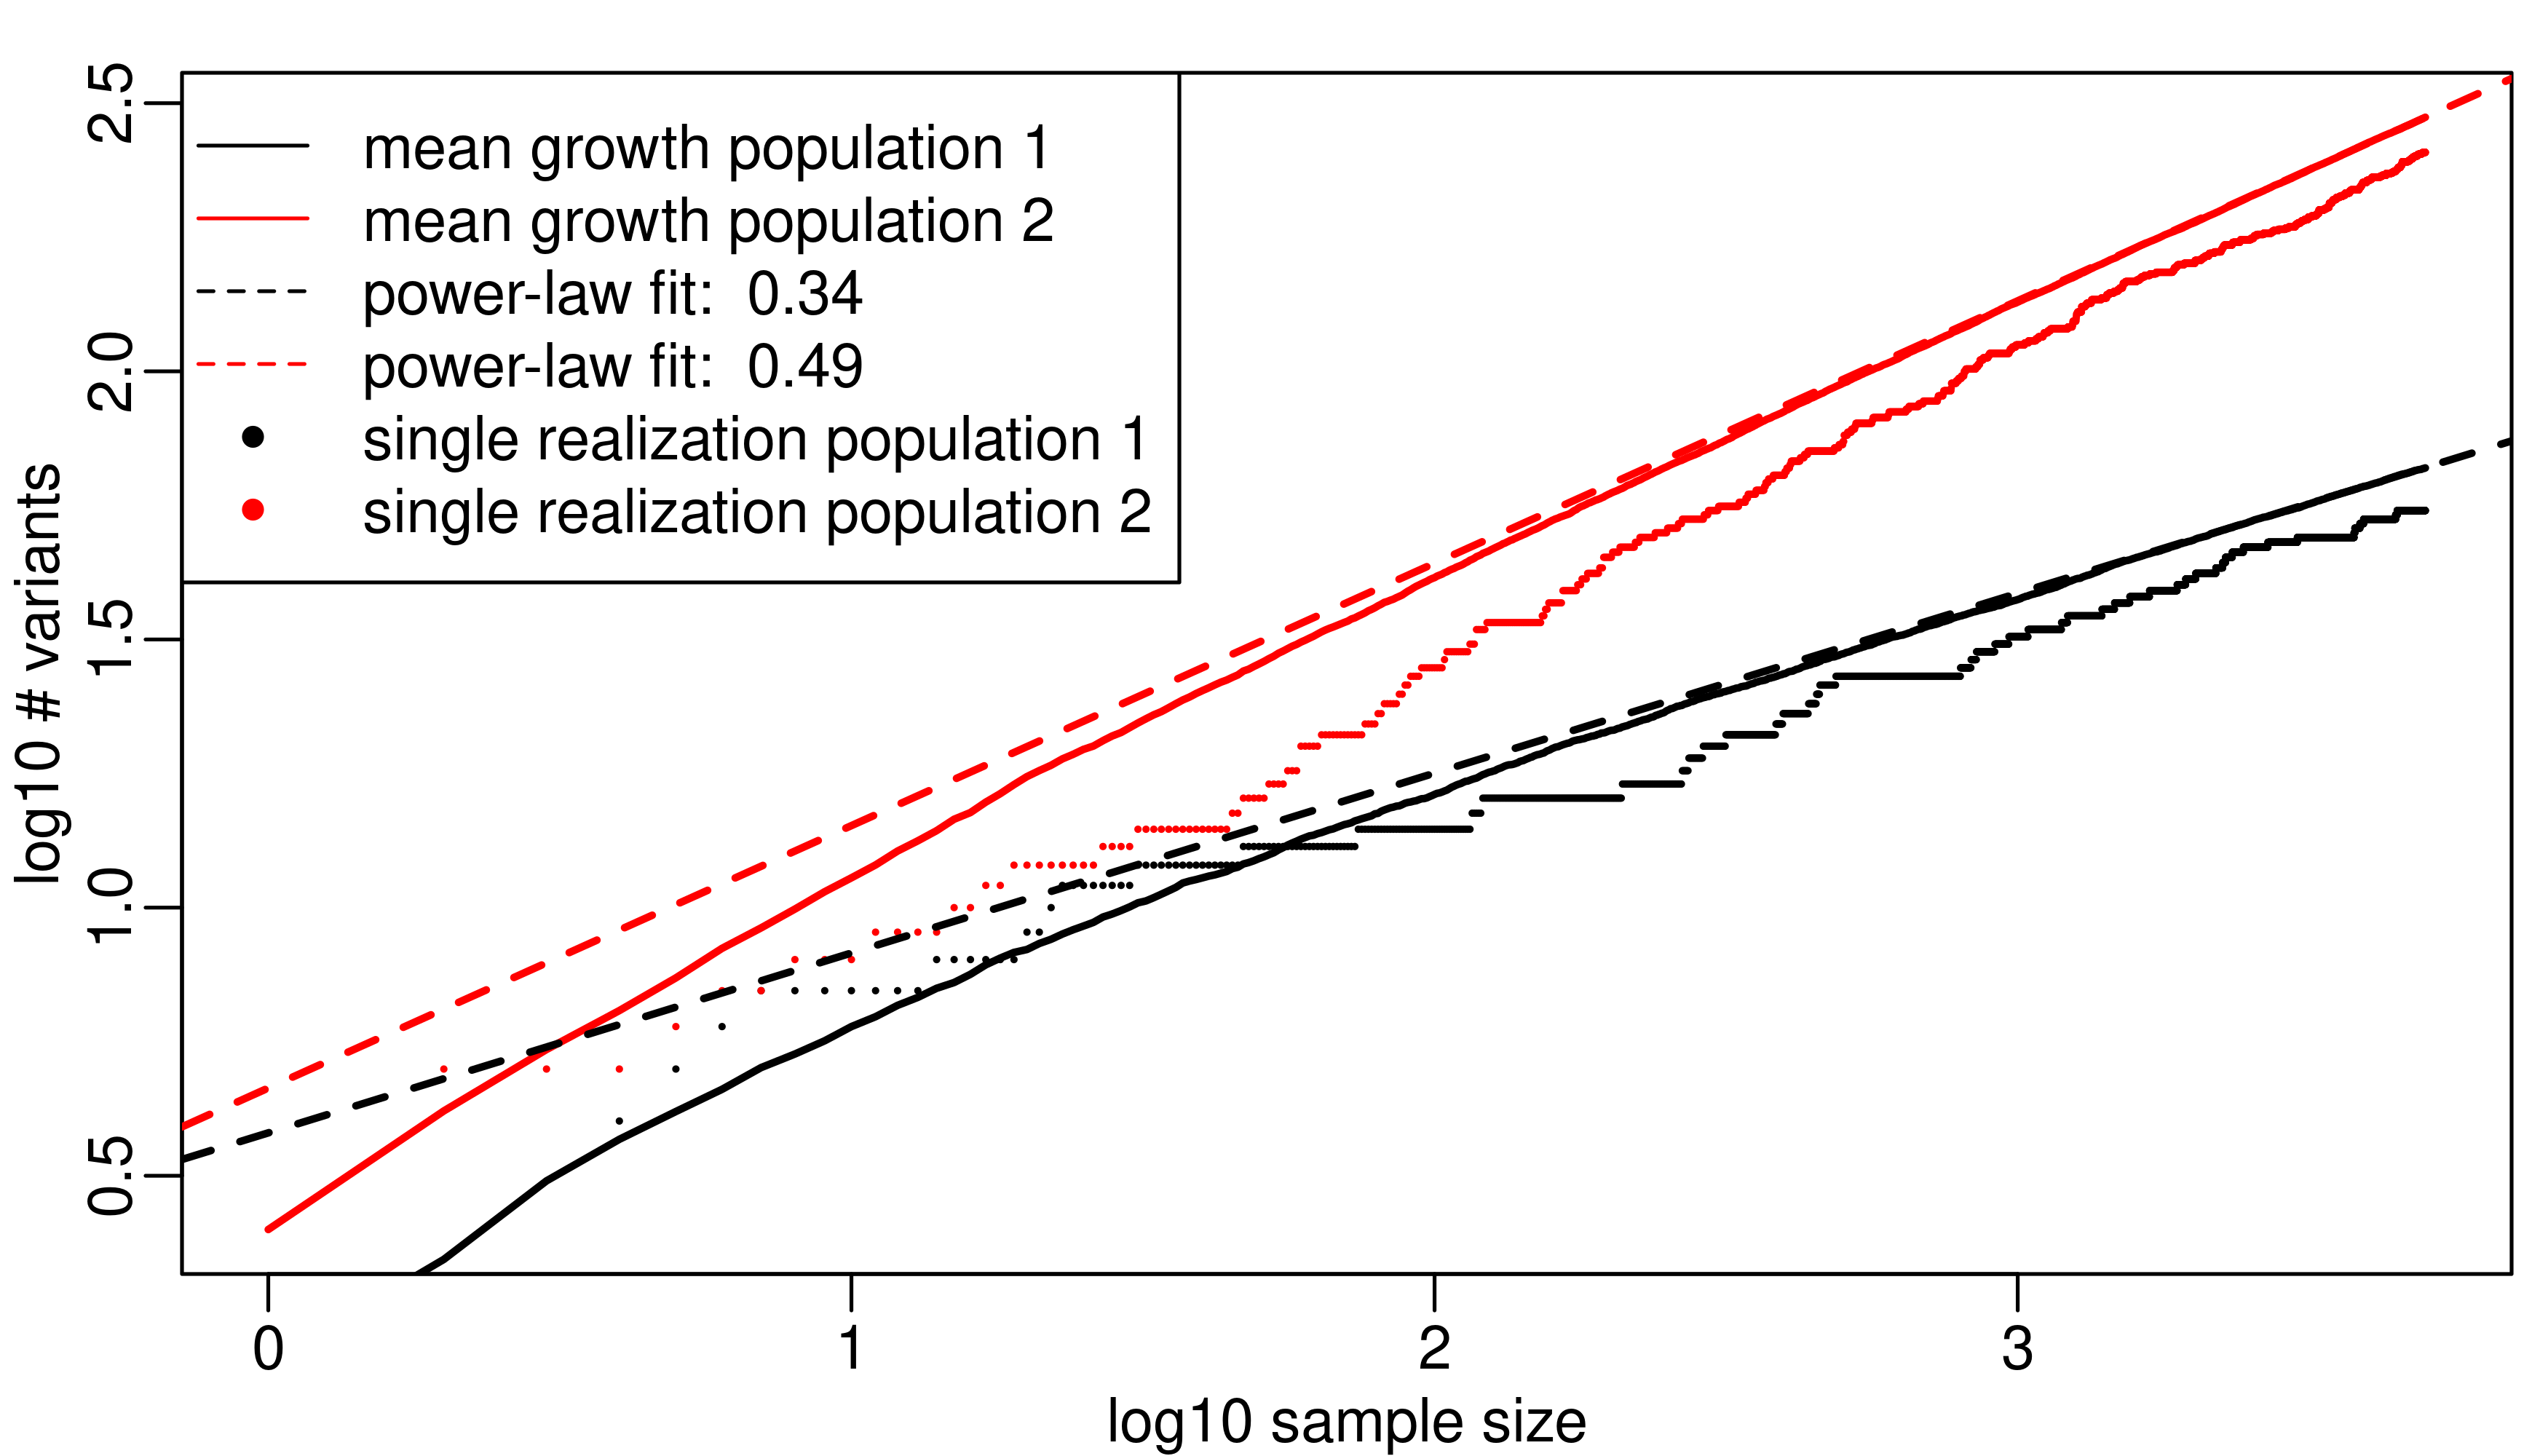
\includegraphics[width = 0.6\textwidth]{Figs/powerlaw_simu_.3_.6_.1.png}
    \caption{ \label{fig:power-law} Illustration of simulated data from our model with $\mass = 10, \rate{1}=0.3, \rate{2}=0.6, \conc{1}=\conc{2}=1, \corr{1}=\corr{2}=0.1$. Under the projection scheme, we take samples from only one population (population 1 in black and 2 in red). The observed number of variants for a given sample size is plotted as a point. To generate a solid curve, we take 100 independent realizations and plot the mean number of observed variants at a particular sample size (and interpolate between sample sizes). To plot the power-law fit, we make a linear least square fit of the log-log plot of the final third of the mean-growth curve and plot the resulting line. %note: log-log plot comes from OLS with both slope and offset parameter
	The fitted power for population 1 is 0.34 and for population 2 is 0.49.}
\end{figure}


%%%
\subsection{The proportional scheme}

We next establish power-law bounds for the expected rate of growth of the number of variants under the proportional scheme. Recall that under the projection scheme, the total number of samples was equal to the number of samples in one of the populations. Under the proportional scheme, the total number of samples will instead be $\samplesize{1} + \samplesize{2} = \lceil (1+\rho) \samplesize{1} \rceil$. We will control the asymptotics by taking $\samplesize{1} \rightarrow \infty$.
 %%%
\begin{myProposition}[Power-law bounds under the proportional scheme] 
    \label{coro:proportional}
	Take the model and hyperparameters as in \Cref{prop:power_law_proj}. Let $\popidx$ be such that $\rate{\popidx} \le \rate{\notpopidx}$, 
	
	For any $\samplesize{1}$, let $\samplesize{2} = \lceil\propt \samplesize{1}\rceil$.
	Then the number of new variants concentrates around its expectation: 
	\[
		\news{\zerovec}{\vecsamplesize} \sim \E \news{\zerovec}{\vecsamplesize}\textrm{ a.s.\ as } \samplesize{1} \to \infty.
	\]
	 Moreover,
	there exist functions $\lowerboundproport, \upperboundproport$ that serve as respective upper and lower bounds on $\E \news{\zerovec}{\vecsamplesize}$,
    \begin{equation*}
        \forall \vecsamplesize,\quad \lowerboundproport(\vecsamplesize)
        		\le \E \news{\zerovec}{\vecsamplesize}
		\le \upperboundproport(\vecsamplesize),
    \end{equation*}
	and that exhibit the asymptotic behavior we describe next. 
	Define $\rate{\notpopidx}'$ as in \Cref{prop:power_law_proj}.
	For any $\smallpositive$ such that $0<\smallpositive\le \min\{\corr{1},\corr{2}\}$, there exist constants $C,C'_{\smallpositive} > 0$ not depending on $\vecsamplesize$ such that 
    \begin{align*}
	\lowerboundproport(\vecsamplesize)
		&\sim C(\samplesize{1}+\samplesize{2})^{\max\{\rate{\popidx},\rate{\notpopidx}'\}}
			\textrm{ \ as } \samplesize{1} \rightarrow \infty \\
    	\textrm{and } \quad \upperboundproport(\vecsamplesize)
		&\sim C'_{\smallpositive}(\samplesize{1}+\samplesize{2})^{\max\{\rate{\popidx},\rate{\notpopidx}\}+\smallpositive} 
			\textrm{ \ as } \samplesize{1} \rightarrow \infty.
    \end{align*}
\end{myProposition}
See Section S8.2 of the Supplementary Material \citep{supplement} for a proof. Essentially we lower bound the total number of variants by the number seen in either population. 
We upper bound the total number of variants by the sum of variants seen in each population; this bound may be somewhat loose since some variants might be shared across the two populations, and hence double counted.  

We next present the special case where the two rate parameters are equal; in this case, the powers in the lower and upper bounds align up to an arbitrary $\smallpositive > 0$ difference.
%%%
\begin{myCorollary}
    \label{coro:proportional_power-law-rate-align}
    Take the same assumptions and constants as \cref{coro:proportional}. Take $\rate{1}=\rate{2}=\rate{}$. Then
    \begin{equation*}
        C(\samplesize{1}+\samplesize{2})^{\rate{}} \sim \lowerboundproport(\vecsamplesize)
        		\le \E \news{\zerovec}{\vecsamplesize}
		\le \upperboundproport(\vecsamplesize) \sim C'_{\smallpositive}(\samplesize{1}+\samplesize{2})^{\rate{}+\smallpositive} \textrm{\ as } \samplesize{1} \to \infty.
    \end{equation*} 
\end{myCorollary}


The result follows directly from \cref{coro:proportional} and noting that, when the rate parameters are equal, we have $\rate{\notpopidx}' = \rate{\notpopidx} = \rate{}$.



\section{Experiments}
\label{sec:experiments}
% !TEX root = ../double_trouble_main.tex

We next check the quality of our predictions experimentally. First we check that our method performs well on well-specified synthetic data, as well as some particular forms of misspecification. Then we see that our method provides high-quality predictions on a real human cancer genetics dataset and a real human genomic dataset. Throughout, we illustrate the advantages of modeling two populations together rather than treating the two populations separately or all from a single population.

\paragraph{Experimental setup.} In all of our experiments, we will have access to a collection of genetic samples for each of two populations (e.g., two types of cancer). Our validation procedure is reminiscent of cross-validation and analogous to the single population validation procedures of \citet{Masoero2022,  zou2016quantifying}. Within each population, we uniformly at random choose a partition of the data into 20 equally-sized blocks. \minorrevision{Since the dataset size may not be a multiple of 20, block sizes in practice may vary by 1. We will elide  small details of this form in the remainder of this section for clarity of exposition. Also, the population genetics data is substantially larger than our other datasets, so --- to avoid a very large pilot size --- we use 30-fold cross-validation in that case (\cref{sec:real_data}).} 

In each of 20 folds, we reserve one block (unique to this fold) to be the pilot data for its corresponding population, so the final pilot sample has size $\vecsamplesize = (\samplesize{1}, \samplesize{2})$. The remaining data will serve as potential follow-up data. Each method has access only to the pilot data (across both populations), and we use the follow-up data (across both populations) to evaluate the accuracy of each method. None of the methods we consider in this paper use ordering information on the pilot data, but to generate all of our figures, we choose an ordering on the pilot data uniformly at random. Likewise, we choose an ordering on the follow-up data uniformly at random. In our figures, we present first the pilot data from population 1, then the pilot data from population 2, then the follow-up data from population 1, then the follow-up data from population 2. We can think of these figures as encapsulating a series of evaluations as follows. We train every method on the full pilot data in populations 1 and 2. Then we progressively test on follow-up sample sizes $\vecfuturesamplesize = (\futuresamplesize{1},\futuresamplesize{2})$ of the following forms: $(1,0), (2,0), \ldots, (19 \samplesize{1},0), (19 \samplesize{1},1), (19 \samplesize{1},2), \ldots, (19 \samplesize{1}, 19 \samplesize{2})$. In this way, we capture a wide range of ratios between follow-up sample sizes across the two populations: from all follow-up data in a single population to a ratio of follow-up sizes that matches the ratio in the pilot.
To summarize our results across all 20 folds, we will show an empirical mean across folds, both for each prediction method as well as for the ground truth. And we will show a shaded one-standard deviation interval for the prediction methods. The ground truth showed very small variation across folds so the interval appears almost invisible. %\tb{ultimately we will say something about ground truth here too once the results are in.} %\tb{Are the intervals for the ground truth very small? can we say something here?}

Recall that we are also interested in predicting the number of $\vecoccurrence$-tons in a follow-up sample of size $\vecfuturesamplesize$ (\cref{eq:news_freq}); that is, we are interested in predicting the number of new variants appearing exactly $\vecoccurrence$ times across the two populations. To evaluate our prediction in this case, we consider just the extreme where we use all possible data in the follow-up. For each value of $\vecoccurrence$ with $\occurrence{1}, \occurrence{2}$ each less than a threshold, we compute the \emph{relative residual}: namely, the signed difference between a method's prediction and the observed value in the reserved follow-up data, normalized by the observed value. We plot an empirical average of this quantity across the folds. We also report the actual observed values and absolute (un-normalized) residuals in Section S7.3 in the Supplementary Material \citep{supplement}, again averaged across the folds.

\paragraph{Comparisons.} To the best of our knowledge, there are no alternative methods for the prediction task we are interested in here. However, there are a number of methods that predict the number of variants in a follow-up given pilot data in a single population~\citep{Masoero2022, chakraborty2019using,gravel2014predicting}. So we consider two natural competitors in our experiments. First, we define the \emph{independent} two-population \revision{application} of a single-population method as follows. Given $\vecsamplesize$ pilot samples and $\vecfuturesamplesize$ follow-up samples, we train the single-population method first on the $\samplesize{1}$ pilot samples from population 1 and predict the number of variants expected in $\futuresamplesize{1}$ follow-up samples from population 1. We separately train the single-population method on the $\samplesize{2}$ samples from population 2 and predict the number of variants expected in $\futuresamplesize{2}$ follow-up samples from population 2. We report the sum of the predicted number of variants across both populations as the final prediction. 
In general, we expect the independent method to overcount the number of variants when there are follow-up samples from both populations. We do not include the independent method below when we compare performance in predicting $\vecoccurrence$-tons. In particular, whenever both elements of $\vecoccurrence$ are strictly positive, the independent method predicts there are zero $\vecoccurrence$-tons. We provide the \revision{prediction, its supporting theory, and how we perform hyperparameter selection} in Section S4.2 of the Supplementary Material of \citep{supplement}. In the real data we analyze at the sizes we consider, this zero prediction is unrealistic; see Figures S8 and S9 in the Supplementary Material \citep{supplement} for the ground-truth real-data $\vecoccurrence$-ton values. %(Also, see \cref{supp-fig:proposed_kton,supp-fig:i3BP_kton,supp-fig:d3BP_kton} for the ground-truth synthetic $\vecoccurrence$-ton values.)

%The independent method essentially assumes each variant is unique to a single population. From that perspective, when $\vecoccurrence = (\occurrence{1},0)$, we can take the population-1 prediction for the number of $\occurrence{1}$-tons and use it as the independent-method prediction for the number of $\vecoccurrence$-tons; an analogous prediction holds when $\occurrence{1} = 0$ and $\occurrence{2} > 0$. Whenever both elements of $\vecoccurrence$ are strictly positive, the independent method predicts there are zero $\vecoccurrence$-tons. In the real data we analyze at the sizes we consider, this zero prediction is unrealistic (see~\Cref{supp-fig:proposed_kton},~\ref{supp-fig:i3BP_kton},~\ref{supp-fig:d3BP_kton} for raw number of $\vecoccurrence$-tons in synthetic experiments and~\Cref{supp-fig:brca_luad_kton},~\ref{supp-fig:seu_bgr_kton} in real data experiments). 

Second, we define the \emph{dependent} two-population \revision{application} of a single-population method. In this case, we train the single-population method on all of the $\samplesize{1} +\samplesize{2}$ pilot samples, as though they are the pilot samples from a single population. To form a prediction on a follow-up sample of size $\vecfuturesamplesize$, we report the prediction on a single-population follow-up of size $\futuresamplesize{1} + \futuresamplesize{2}$. 
In general, we expect the dependent method to struggle when both (a) the two populations exhibit notably different variant growth rates and (b) the ratio of populations in the follow-up does not closely mirror the pilot \revision{because this mismatch exacerbates prediction errors. For example, if one population contains many rare variants while the other does not, changing the sampling proportions between pilot and follow-up will substantially impact variant discovery rates in ways the homogeneous model cannot account for.}
To predict the number of $\vecoccurrence$-tons, we predict the number of variants, conditional on the pilot, that we would expect to see $\occurrence{1}$ times out of $\futuresamplesize{1}$ follow-up samples and also $\occurrence{2}$ times out of $\futuresamplesize{2}$ distinct follow-up samples (all from the same assumed single population). For single-population methods that do not provide $\occurrence{}$-ton predictions (for scalar $\occurrence{}$), we will therefore not be able to provide $\vecoccurrence$-ton predictions in the dependent \revision{application}. 
However, we are able to provide $\vecoccurrence$-ton predictions for the special case of the single-population 3BP method due to \citet{Masoero2022}.
\internal{In particular, in Section S4.1 of the Supplementary Material \citep{supplement}, we describe how we modify \citet{Masoero2022} to predict vector-valued $\vecoccurrence$-tons; we provide theory analogous to \cref{prop:predict_kr_tons} and describe the method we employ to fit the hyperparameters}.
%\internal{see Section S4.1 of the Supplementary Material \citep{supplement} for a discussion on modifying \citet{Masoero2022} to predict vector values $\vecoccurrence$-tons, including supporting theory and the method employed to fit the hyperparameters}.

Since there are many single-population methods, in general we will select just one single-population method to use when reporting the independent and dependent results. In each case, we will try to use the single-population method that is best in a relevant sense, which we make precise in each case below.


\subsection{Synthetic experiments}
\label{sec:simulation}
% !TEX root = ../double_trouble_main.tex

We first confirm that our method is able to predict well on data simulated from our own model (\cref{eq:proposed_prior}), as a check on our methodology before moving to real data. To that end, we generate 500 data points in each of two populations; we describe the simulation procedure in more detail in~Section S6 of the Supplementary Material \citep{supplement}. So, in each of our 20 folds, the pilot data has size $\vecsamplesize = (25,25)$.

We simulate two different datasets from our model (\cref{eq:proposed_prior}); we choose the hyperparameters to reflect a range of growth rates, sample sizes, and correlations between the two populations in each case. We choose hyperparameters $\allhyper := (\mass, \rate{1},\rate{2}, \corr{1},\corr{2}, \conc{1},\conc{2}) = (100,0.4,0.6,0.5,0.5,1,1)$ for the first dataset and $\allhyper = (1,0.8,0.7,0.5,0.5,1,1)$ for the second dataset. We choose these values for qualitative matches with the observed variant growth in the GnomAD dataset (\cref{fig:pop_gen}) and cancer dataset (\cref{fig:cancer}), respectively. 

The results in \cref{fig:proposed} demonstrate that our method outperforms two potential baselines. Since here all of our data is simulated from our two-population BNP model, we use a single-population BNP model to form our baselines; namely, we compare to the independent and dependent two-population applications of the 3BP approach due to \citet{Masoero2022}. \internal{First, consider the simulation in the upper row of plots.} We see in the upper left plot in \cref{fig:proposed} that our method (solid red line) much more closely matches the behavior of the ground truth (dashed black line) than either the independent (dotted green line) or dependent (dash-dot blue line) applications. As expected, the independent application dramatically overcounts the number of variants in the second follow-up population. Also as expected, the dependent application performs well when the pilot and follow-up proportions are in agreement (at the largest sample size) but misestimates the number of variants elsewhere. By contrast, our method is able to capture the different behaviors of the two populations and account for any shared variants.

 In the lower left corner, the independent application of the 3BP performs the best; its mean line is closest to the ground truth, and its prediction exhibits the smallest variation (shaded range) across folds. Importantly, \internal{we can infer from the lower center plot that} there are extremely few shared variants in \internal{the simulation for the lower row}; see Section S7.3 of the Supplementary Material \citep{supplement} \internal{for raw observed and predicted counts.} That is, \internal{in the simulation for the lower row of plots,} the assumption of the independent application is very close to being correct. So, following Bayesian Occam's Razor \citep[ch.~28 p.~343]{mackaybook}, we expect better performance from the simpler model (the independent application) when its more stringent assumptions are true. That being said, our proposed model still performs well here; its mean line is also very close to the ground truth, by contrast to the dependent application. We conclude that our method is able to handle prediction of the number of new variants under a variety of two-population behaviors --- while the independent application is limited to the special cases where the two populations are known a priori to behave independently.

\begin{figure}[htp]
    \centering
    \includegraphics[width = 0.9\textwidth]{Figs/n3BP_20fold.png}
    \includegraphics[width = 0.9\textwidth]{Figs/n3BP_fast_20fold.png}
    \caption{Predictions when data is sampled from our model (\cref{eq:proposed_prior}). Each row corresponds to a simulated dataset (\cref{sec:simulation}). \emph{Left}: %The dashed black line shows the observed number of variants as a function of the sample number.
    The samples (horizontal axis) appear in the following order: pilot from population 1, pilot from population 2, follow-up from population 1, follow-up from population 2. A vertical dashed gray line separates the two populations in the pilot and follow-up, respectively. Vertical gray shading covers the pilot data. In the follow-up region, we plot mean (lines) and 1 standard deviation intervals (shaded regions) from ground truth (dashed black; also appears for the pilot) and three methods: our proposed method (solid red), the dependent version of the single-population 3BP (dash-dot blue), and the independent version of the 3BP (dotted green). \emph{Center and Right}: For each $\vecoccurrence$ with component values up to 10, we plot the relative residual for predictions from our method (right) and the dependent 3BP (center). \revision{Note: color scales are dataset-specific.} A square is gray when the observed value is strictly less than 2 in at least one fold or $\vecoccurrence = (0,0)$. 
    }
    \label{fig:proposed}
\end{figure}

From the center and right plots in \cref{fig:proposed}, we also see that our method provides better estimates of the numbers of various $\vecoccurrence$-tons. Recall that the independent application predicts zero for anything except private $\vecoccurrence$-tons, and we see that there are in fact non-trivial counts of shared $\vecoccurrence$-tons in the first data set. Given this limitation of the independent application, we focus on plotting results for our method and the dependent application. Darker colors indicate more erroneous predictions, so we conclude in both datasets that our method is providing more accurate predictions than the dependent 3BP application. Note that the observed numbers of $\vecoccurrence$-tons vary dramatically across $\vecoccurrence$ values. So generally we expect more noise in the upper right of our plots of $\vecoccurrence$-tons --- and should therefore take care not to treat every square in these plots equally. We can see the actual observation values for the two datasets in \internal{Fig. S5 (Section~S7.3)} of the Supplementary Material \citep{supplement}; in particular, for the first dataset, the observed number of $\vecoccurrence$-tons varies from an average (across folds) of 1161.2 at $(0,1)$ to 0 at various locations, e.g. (8,3), (10,4), and (7,7) (see the gray boxes in the upper left panel of \internal{Fig. S5 (Section~S7.3)} of the Supplementary Material \citep{supplement}).  We see similar behavior in the real data, as we describe below.

We check that our method is able to handle datasets generated from the (mis-specified) assumptions of the independent and dependent 3BP applications in Sections S7.1 and S7.5 of the Supplementary Material \citep{supplement}; \internal{in particular, in S7.5, we investigate a case where the data is generated from a dependent 3BP where the number of variants grows slowly, and using the independent 3BP for inference results in severe double counting of variants --- but our method continues to work well.}



\subsection{Real data}
\label{sec:real_data}
% !TEX root = ../double_trouble_main.tex

We next show that our method performs well on a real dataset in cancer genomics and semi-synthetic dataset in population genetics. We confirm that our method performs better than the independent and dependent applications of one-population methods.

\paragraph{Comparisons.} For the real datasets, we find that different one-population methods exhibit substantially different performance for different types of data. So, for each type of data (cancer, population genetics), we test a variety of different one-population methods. In Section S7.2 of the Supplementary Material \citep{supplement}, we compare them on the one-population task and choose the best-performing method to serve as the comparison (via independent and dependent applications) for our two-population method. \internal{In particular, we choose the one-population method with the lowest root mean squared error of the prediction curve for the number of variants; here, we take the mean across all values of the follow-up sample size (up to the largest value), and we note that this value depends on our choice of ordering of the data points.} For one-population methods, we consider the fourth-order jackknife \citep{burnham1978estimation, gravel2014predicting}, the Good-Toulmin estimator \citep{Orlitsky2016,chakraborty2019using}, linear programming \citep{zou2016quantifying}, the 3BP approach of \citet{Masoero2022}, and the scaled process of \citet{Camerlenghi2021}.


\paragraph{Two cancer genomic datasets.}
%
In cancer genomics, biologists are actively searching for (rare) shared genetic variants across cancer types that might lend insight into common causes of different cancers \citep{bojesen2013multiple, rashkin2020pan}. We next show that both our method and the independent application perform well at predicting the number of new variants, while the dependent application performs poorly. But unlike the independent application, our method is able to predict the (non-trivial) number of shared variants across populations -- and provides a better prediction than the dependent application.

In these experiments, we use the cancer genome atlas (TCGA) and MSK-IMPACT datasets \citep{cancer2008comprehensive, cancer2013cancer, cheng2015memorial}. 
We used the same processing as in \citet{chakraborty2019using} and \citet{Masoero2022}. 

To form our two populations, we focus on the two types of cancer with the largest numbers of samples; in each dataset, the resulting two types of cancer are lung cancer and breast cancer. In the MSK-IMPACT dataset, there are total of 749 lung cancer samples and 1532 breast cancer samples. In the TCGA dataset, there are total of 492 lung cancer samples and 811 breast cancer samples. So the pilot sizes are challenging in each case: 38, 57, 24, and 40, respectively.
%
For each population (lung cancer, breast cancer) in each dataset (TCGA, MSK-IMPACT), we find that the best-performing one-population method is the 3BP (Section S7.2 of the Supplementary Material \citep{supplement}). So we compare to the independent and dependent one-population applications of the 3BP in this analysis.



\begin{figure}[htp]
    \centering
    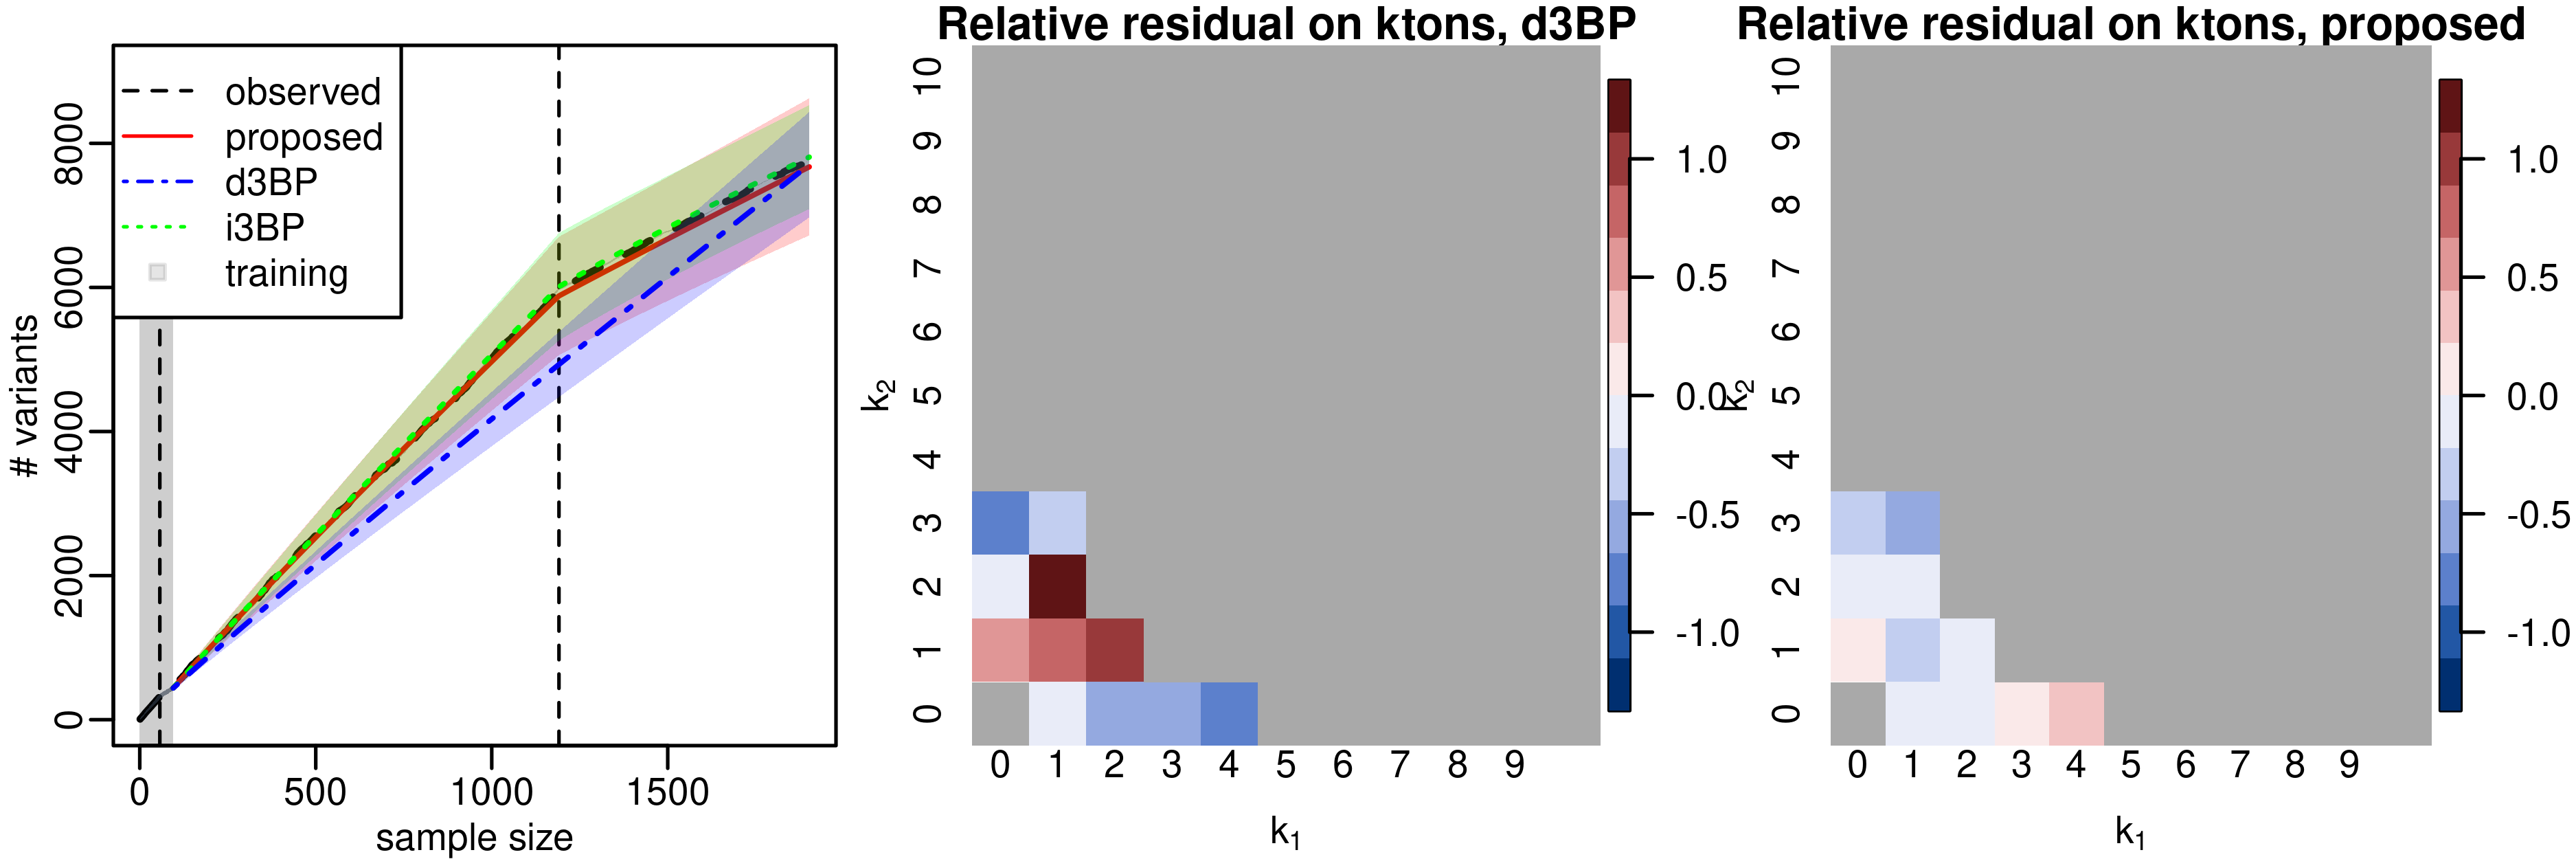
\includegraphics[width = 0.9\textwidth]{Figs/BIDC_LA2_20fold.png}
    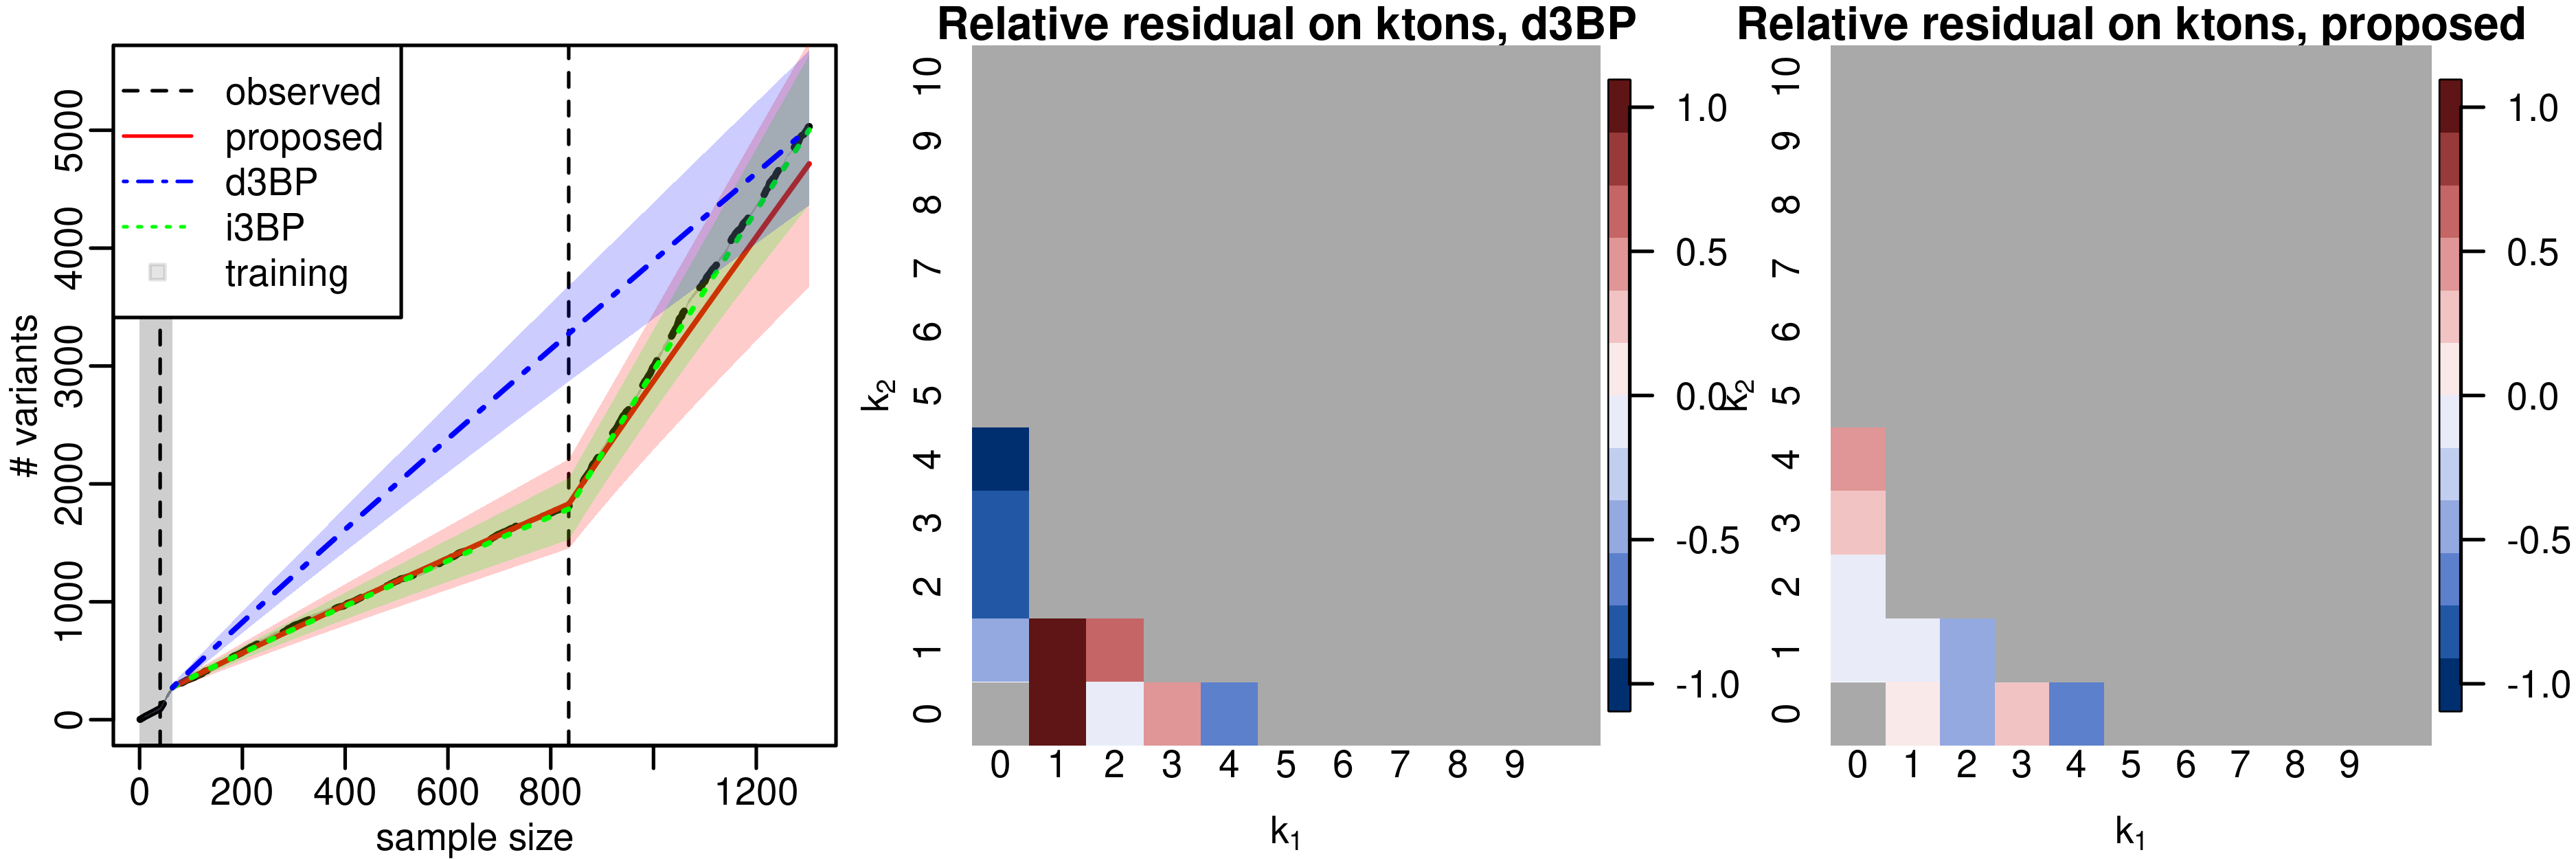
\includegraphics[width = 0.9\textwidth]{Figs/BRCA_LUAD_20fold.png}
    \caption{Predictions for the cancer genomics data. The rows correspond to datasets (upper: MSK-IMPACT, lower: TCGA). Population 1 is breast cancer, and population 2 is lung cancer. Other details of the plots are as in \cref{fig:proposed}.
    }
    \label{fig:cancer}
\end{figure}

The results in \cref{fig:cancer} demonstrate that our method outperforms the two one-population baselines. In particular, both our method and the independent application agree closely with the ground truth number of new variants across the various follow-up sizes (left panels). Indeed, we expect a low level of sharing between cancer types since most variants in cancer are \textit{de novo} variants -- not subject to the natural selection that might make variants more likely to be shared across populations. As expected the dependent application agrees with ground truth when the composition of the follow-up matches the pilot, but its predictions can be very far from the ground truth for other follow-up sizes. In the center and right plots, we see that there are still a number of shared variants with non-trivial counts in the ground truth; see also~Figure S8 of the Supplementary Material \citep{supplement} for direct plots of the ground truth. The independent application is unable to predict such counts. And while the dependent application can predict a non-zero number in these cases, we see from the center and right plots in \cref{fig:cancer} that our method's predictions are more accurate. Overall then, our method is the only one able to provide both useful predictions of the numbers of variants in a follow-up as well as useful predictions of the number of shared variants across populations in the follow-up.


\paragraph{A semi-synthetic population genetics dataset.}
%\label{sec:gnomad}

For population genetics, we use the GnomAD dataset \citep{karczewski2020mutational}. The dataset provides variant frequencies, but it does not provide exact variant data for each sample. So we take the semi-synthetic approach of \citet{Masoero2022}; namely, for each individual, we independently sample the presence of each variant according to the reported frequency of that variant in the data. In general, prediction is more challenging (a) when the pilot is small in absolute terms since less trend information is available 
and (b) when the follow-up is as large as possible since we have a priori more possibility for any observed trend to break down. To accomplish goal (b), we choose large populations: Korean (1909 samples), Bulgarian (1335), and Southern European (5752). We then choose 30 folds to ensure smaller pilots 
(64, 45, and 192, respectively), per goal (a).

For each population (Korean, Bulgarian, Southern European), we compare performance of the one-population \internal{methods listed at the start of} \cref{sec:real_data}; see Section S7.2 of the Supplementary Material \citep{supplement} \internal{for results}. For each population in this case, we find that the fourth-order jackknife (4JK) \internal{is the best performer}. So we use the 4JK for the independent and dependent one-population applications in this analysis.

The results in \cref{fig:pop_gen} demonstrate that our method outperforms the two one-population methods at predicting the number of new variants in a follow-up. When the follow-up composition matches the pilot (the most favorable case for the dependent application), our method is at least on par with the dependent one-population application at predicting the number of shared variants in a follow-up. 
We see in the upper left plot that the dependent application miscounts variants when the composition of the follow-up differs from the pilot. The independent application predicts the first population well but double counts shared variants when the second population appears in the follow-up. In the lower left, the two populations are more similar, so the dependent application performs reasonably; the independent application, though, double counts shared variants in the second population in the follow-up. In both examples, our method tracks closely with ground truth. 

In the upper center plot, we see that the dependent one-population application can be over an order of magnitude off in its predictions. In the upper right plot, we see that our method is much closer to ground truth across the $\vecoccurrence$ values here. Unlike in the cancer data case, the ground truth at all $\vecoccurrence$ values in this plot is substantially greater than zero; see Figure S8 of the Supplementary Material \citep{supplement} for more information about the ground-truth counts. In particular, the signed residual plot in Figure S8 of the Supplementary Material \citep{supplement} shows that the dependent application is providing an overestimate along the diagonal. Indeed, we expect that the Korean and Bulgarian populations have little overlap and thus few shared variants -- whereas the dependent application assumes they are the same population. Conversely, in the lower center and right plots, we see that our method is often farther from the ground truth than the dependent application. We note that the magnitude of the error is smaller than in the upper plots, but it is still quite high (larger than 100\%). It may be that the complex history between the related Southern European and Bulgarian populations cannot be captured by the simple models we consider here.  We reiterate that the independent application predicts zero for all $\vecoccurrence$ values that do not have a zero component and thus fails to predict all such values in these examples.






\begin{figure}[htp]
    \centering
    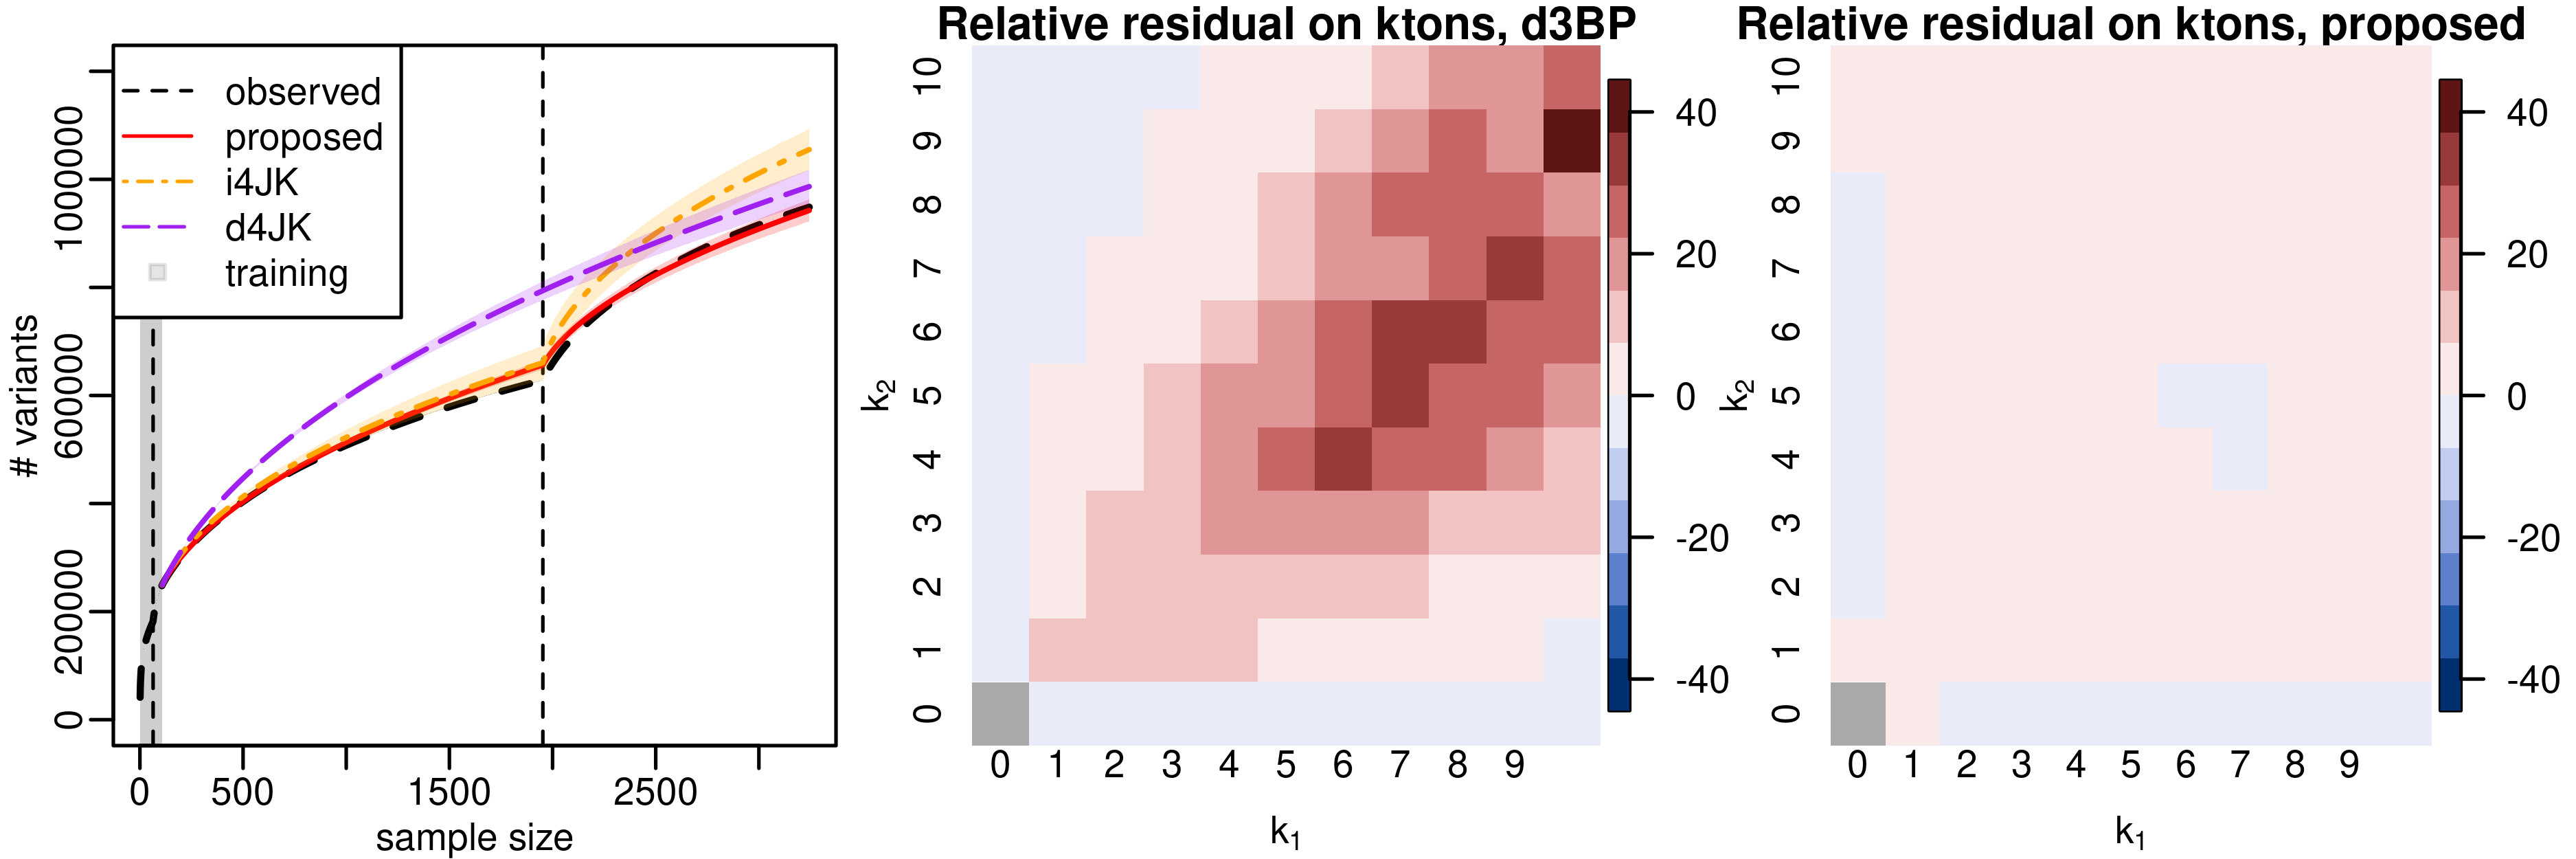
\includegraphics[width = 0.9\textwidth]{Figs/kor_bgr_30fold.png}
    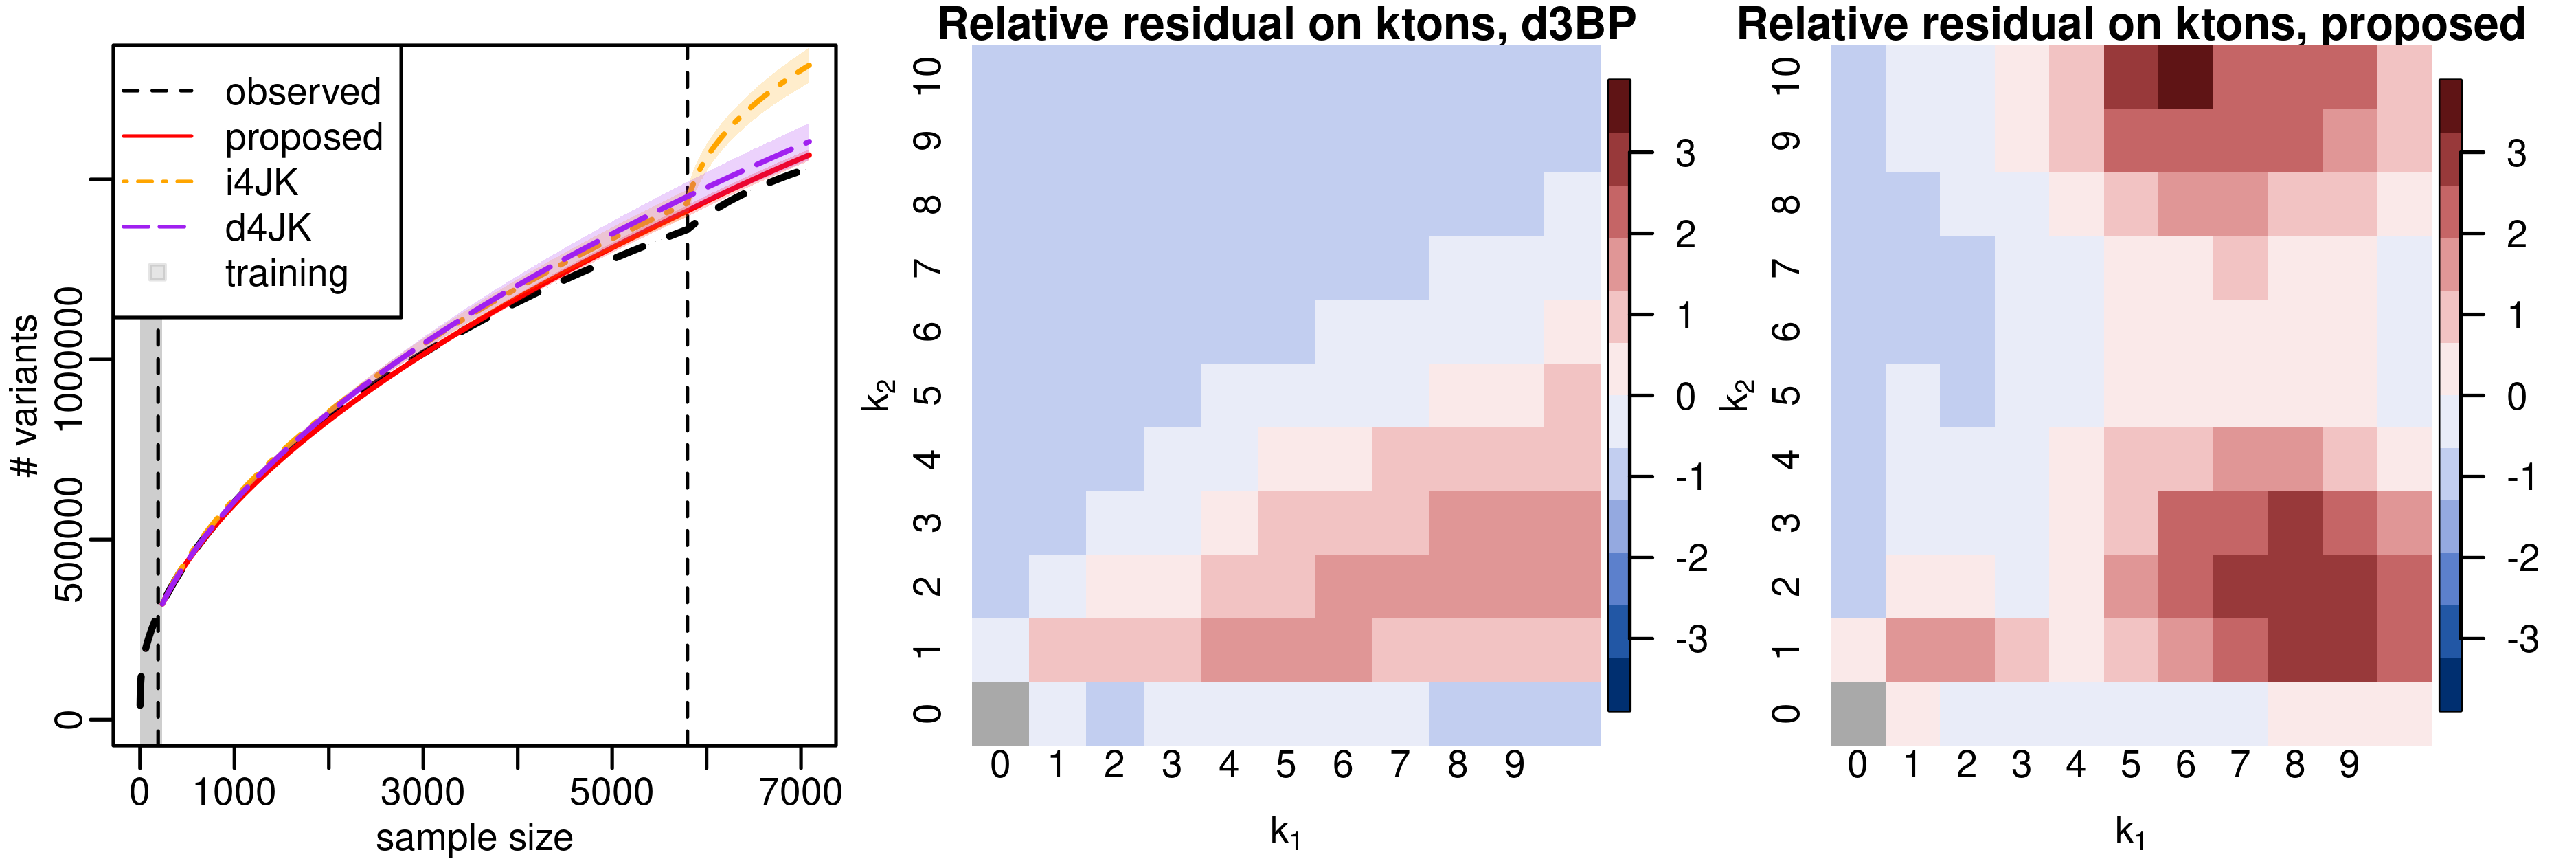
\includegraphics[width = 0.9\textwidth]{Figs/seu_bgr_30fold.png}
    \caption{Predictions for the gnomAD data. The rows correspond to datasets (upper: Korean--Bulgarian, lower: Southern European--Bulgarian). In particular, in the top row, population 1 is Korean, and population 2 is Bulgarian. In the bottom row, population 1 is Southern European, and population 2 is Bulgarian. Other details of the plots are as in \cref{fig:proposed}. We highlight the very different color scales between the upper and lower rows.
    }
   \label{fig:pop_gen}
\end{figure}



\section{Discussion}
\label{sec:discussion}
We proposed a novel approach to estimating the number of new genetic variants that will be observed in a follow-up sequencing study of two potentially heterogeneous populations.

Several opportunities remain for future work. First, we rely on numerical integration for our predictions. Even in the two-population case, these computations can be somewhat expensive. 
\internal{We observe in \cref{app:extension}} that the form of our rate measure in \cref{eq:proposed_prior} is straightforward to extend to more populations. However, 
we expect further computational (and statistical) challenges when considering higher numbers of populations. %We suspect that alternative approaches may prove fruitful.
In addition, we explored only one possible option for generalizing the beta process to higher dimensions. Although our experiments validated our approach, even better performance might be possible with an alternative model -- especially one carefully aligned with biological prior knowledge. \revision{For instance, one drawback of our current rate measure (\cref{eq:proposed_prior}) is its evident asymmetry across populations. It remains to be seen if a symmetric rate measure might be designed to have at least as many desirable properties as \cref{eq:proposed_prior} enjoys (including conjugacy, \cref{req:finite_mean,req:inf_mass}, power law growth rates, empirical performance).}


\begin{acks}[Acknowledgments]
    YS and TB were supported in part by the DARPA I2O LwLL program, an NSF Career Award, and an ONR Early Career Grant. JGS was supported by NIH grant R35GM137758 to Michael D. Edge. 
    The authors acknowledge the MIT SuperCloud and Lincoln Laboratory Supercomputing Center for providing HPC resources that have contributed to the research results reported within this paper. \revision{We thank the anonymous referees for comments that led to substantial improvements of our paper.}

\end{acks}
    
%\begin{funding}[Funding]
%    YS and TB were supported in part by the DARPA I2O LwLL program, an NSF Career Award, and an ONR Early Career Grant. JGS was supported by NIH grant R35GM137758 to Michael D. Edge. 
%\end{funding}

%%%%%%%%%%%%%%%%%%%%%%%%%%%%%%%%%%%%%%%%%%%%%%
%% Supplementary Material, if any, should   %%
%% be provided in {supplement} environment  %%
%% with title and short description.        %%
%%%%%%%%%%%%%%%%%%%%%%%%%%%%%%%%%%%%%%%%%%%%%%
\begin{supplement}
\stitle{We here describe the content of supplementary Material for ``Double trouble: Predicting new variant counts across two heterogeneous populations''}
\sdescription{
\internal{
The supplement contains mathematical proofs of the theorems presented in the main text and additional experiments. 
In particular: 
Section S1 contains the proof for our impossibility result (\cref{prop:incomp} in \cref{sec:cant_have_it_all}).
Section S2 contains the proof that our proposed prior satisfies \cref{req:finite_mean,req:inf_mass}.
Section S3 contains the proof that our proposed prior forms a conjugate family to the Bernoulli likelihood process.
Section S4 contains a full derivation of the inference procedure we adopt for single population methods.
Section S5 contains details on the inference procedure we adopt to implement our proposed method.
Section S6 contains details on the setup we adopt for our simulation studies.
Section S7 contains additional results for both simulated and real data.
Section S8 contains proofs of the asymptotic results presented in \cref{sec:powerlaw}.
}}
\end{supplement}
%\begin{supplement}
%\stitle{Title of Supplement B}
%\sdescription{Short description of Supplement B.}
%\end{supplement}

%The following are some other citations to check that the bibliographc style
%file is working correctly: \citet{akaike}, \citet*{akivarsq}, \citet{dyke},
%\citet{greene}, \citet*{kstuart}, \citet{hilbetech}, \citet{hilbe},
%\citet{hilbeglm}, \citet{maddalacntrsq}, and \citet*{companion}.  


\bibliographystyle{ba}
\bibliography{refs}




\end{document}

